\documentclass[12pt,a4paper]{report}
% Required packages
\usepackage[utf8]{inputenc}
\usepackage[T1]{fontenc}
\usepackage{graphicx}
\usepackage{setspace}
\usepackage{titlesec}
\usepackage{tocloft}
\usepackage{fancyhdr}
\usepackage[margin=1in]{geometry}
\usepackage[normalem]{ulem}
\usepackage{times}
\usepackage{amsmath}
\usepackage{xcolor}
\usepackage{microtype}
\usepackage{ragged2e} % Alignment - load after microtype
\usepackage{enumitem}
\usepackage{hyperref} % Load hyperref last


% Set all list items to 12pt font
\setlist[itemize]{label=$\bullet$, font=\fontsize{12}{14}\selectfont, before=\fontsize{12}{14}\selectfont}
\setlist[enumerate]{font=\fontsize{12}{14}\selectfont, before=\fontsize{12}{14}\selectfont}
\setlist{font=\fontsize{12}{14}\selectfont, before=\fontsize{12}{14}\selectfont}


% Setup hyperref package
\hypersetup{
    colorlinks=true,
    linkcolor=black,
    citecolor=red,
    filecolor=magenta,
    urlcolor=cyan,
}

\emergencystretch=2em
\sloppy

% Setting up line spacing (1.5)
\setstretch{1.5}

% Setting up headers and footers
\pagestyle{fancy}
\fancyhf{}
\fancyfoot[C]{\thepage}
\renewcommand{\headrulewidth}{0pt}
\renewcommand{\footrulewidth}{0pt}

% Title formatting for Chapter Numbers
\titleformat{\chapter}[display]
  {\normalfont\fontsize{14}{16}\bfseries\centering}
  {\MakeUppercase{\chaptertitlename\ \thechapter}}
  {10pt}
  {\MakeUppercase}
\titlespacing{\chapter}{0pt}{-30pt}{20pt}



% Section formatting - 12pt Times Roman Bold
\titleformat{\section}
  {\normalfont\fontfamily{ptm}\fontsize{12}{14}\selectfont\bfseries}{\thesection}{1em}{}

% Subsection formatting - 12pt Times Roman Bold
\titleformat{\subsection}
  {\normalfont\fontfamily{ptm}\fontsize{12}{14}\selectfont\bfseries}{\thesubsection}{1em}{}

% Subsubsection formatting - 12pt Times Roman Bold
\titleformat{\subsubsection}
  {\normalfont\fontfamily{ptm}\fontsize{12}{14}\selectfont\bfseries}{\thesubsubsection}{1em}{}

% Set paragraph alignment to justified
\AtBeginDocument{\justifying}
\setlength{\parindent}{15pt}

% Add space between table caption and table
\usepackage{caption}
\captionsetup[table]{skip=10pt}

% Table of Contents styling
\renewcommand{\contentsname}{Table of Contents}
\renewcommand{\cfttoctitlefont}{\hfill\Large\bfseries}
\renewcommand{\cftaftertoctitle}{\hfill}
\renewcommand{\cftchapfont}{\bfseries}
\renewcommand{\cftchappagefont}{\bfseries}

% Add custom entries to TOC
\newcommand{\addtotocnonum}[2]{%
  \addcontentsline{toc}{#1}{#2}%
}

% List of Figures styling
\renewcommand{\cftloftitlefont}{\hfill\Large\bfseries}
\renewcommand{\cftafterloftitle}{\hfill}

% List of Tables styling
\renewcommand{\cftlottitlefont}{\hfill\Large\bfseries}
\renewcommand{\cftafterlottitle}{\hfill}

% Begin the document
\begin{document}

% Title Page
\thispagestyle{empty}
\begin{center}
    \vspace{-0.3cm}

    {\fontsize{12}{19}\selectfont\textbf{MINOR PROJECT REPORT}}\\
    \vspace{0.2cm}

    {\fontsize{12}{17}\selectfont\textit{On}}\\
    \vspace{0.1cm}

    {\fontsize{12}{19}\selectfont\textbf{"Customer Personality Segmentation System using Machine Learning"}}\\
    \vspace{0.5cm}

    {\fontsize{12}{14}\selectfont\textit{Submitted in partial fulfillment of the requirements for the award of}}\\
    \vspace{0.1cm}

    {\fontsize{12}{17}\selectfont\textbf{Bachelor of Technology (B.Tech)}}\\
    \vspace{0.1cm}

    {\fontsize{12}{14}\selectfont In the department of}\\
    \vspace{0.1cm}

    {\fontsize{12}{17}\selectfont\textbf{Computer Science \& Engineering}}\\

    % Logo
    \vspace{0.3cm}
    \includegraphics[width=4.5cm]{au.png}\\
    \vspace{0.4cm}

    {\fontsize{12}{14}\selectfont Submitted by:}
    \vspace{0cm}

    {\fontsize{12}{14}\selectfont\textbf{Koushik Mondal (UG/02/BTCSE/2022/006)}}\\
    {\fontsize{12}{14}\selectfont\textbf{Kalyan Ghosh (UG/02/BTCSE/2022/007)}}\\
    {\fontsize{12}{14}\selectfont\textbf{Imran Nazim Mallik (UG/03/BTCSE/2022/009)}}\\
    {\fontsize{12}{14}\selectfont\textbf{Bhabajyati Bhattacharjya (UG/02/BTCSE/2022/011)}}\\

    \vspace{1cm}
    
{\fontsize{12}{14}\selectfont Under the Guidance of}\\
    \vspace{0cm}

    {\fontsize{12}{16}\selectfont\textbf{Dr. Samik Datta}} \\
    {\fontsize{12}{14}\selectfont\textbf{(Assistant Professor)}}\\

    \vspace{1cm}
    {\fontsize{12}{16}\selectfont\textbf{School of Engineering \& Technology}}\\
    {\fontsize{12}{16}\selectfont\textbf{ADAMAS University, Kolkata, West Bengal}}\\
    \vspace{0.2cm}
    {\fontsize{12}{14}\selectfont\textbf{Aug 2025 - Dec 2025}}
\end{center}
\newpage

\pagenumbering{roman}
\addcontentsline{toc}{chapter}{Title Page}

%----------------------------------
% Certificate
%----------------------------------
\thispagestyle{plain}
\addcontentsline{toc}{chapter}{CERTIFICATE}
\begin{center}
    \Large{\fontsize{14}{16}\selectfont\textbf{CERTIFICATE}}
\end{center}
\vspace{1.5cm}
\noindent This is to certify that the project report entitled \textbf{"Customer Personality Segmentation System using Machine Learning"}, submitted to the School of Engineering \& Technology (SOET), ADAMAS UNIVERSITY in partial fulfillment for the completion of Semester – 7th of the degree of Bachelor of Technology in the department of Computer Science \& Engineering, is a record of bonafide work carried out by \textbf{ Koushik Mondal,UG/02/BTCSE/2022/006, Kalyan Ghosh,UG/02/BTCSE/2022/007, Imran Nazim Mallik,UG/02/BTCSE/2022/009, Bhabajyati Bhattacharjya,UG/02/BTCSE/2022/011,}, under our guidance.
\vspace{1cm}

\noindent All help received by us from various sources has been duly acknowledged.

\noindent No part of this report has been submitted elsewhere for the award of any other degree.
\vspace{2cm}
\begin{center}
    \underline{\hspace{5cm}}\\
    \textbf{Dr. Samik Datta}\\
    \textbf{(Assistant Professor)}

    \vspace{1cm}
    \underline{\hspace{5cm}}\\ 
    \textbf{Sayantan Singha Roy / Aninda Kundu}\\
    \textbf{(Project Coordinator)}

    \vspace{1cm}
    \underline{\hspace{5cm}}\\
    \textbf{Dr. Sajal Saha}\\
    \textbf{(Asso. Dean \& HOD CSE)}
\end{center}
\newpage

%----------------------------------
% Acknowledgement
%----------------------------------
\thispagestyle{plain}
\addcontentsline{toc}{chapter}{Acknowledgement}
\begin{center}
    \Large{\fontsize{14}{16}\selectfont\textbf{Acknowledgement}}
\end{center}
\vspace{1.5cm}

\justifying
\noindent The satisfaction and euphoria that accompany the successful completion of any task would be incomplete without the mentioning of the people whose constant guidance and encouragement made it possible. I take pleasure in presenting before you, my project, which is the result of a studied blend of both research and knowledge.

\vspace{0.5cm}

\noindent I express my earnest gratitude to \textbf{Dr. Samik Datta (Assistant Professor)}, Department of CSE, for his/her constant support, encouragement, and guidance. I am grateful for his/her cooperation and valuable suggestions.

\vspace{0.5cm}

\noindent Finally, I express my gratitude to all other members who are involved either directly or indirectly for the completion of this project.
\newpage

%----------------------------------
% Declaration
%----------------------------------
\thispagestyle{plain}
\addcontentsline{toc}{chapter}{DECLARATION}
\begin{center}
    \Large{\fontsize{14}{16}\selectfont\textbf{DECLARATION}}
\end{center}
\vspace{1.5cm}
\noindent I, the undersigned, declare that the project entitled \textbf{"Customer Personality Segmentation System using Machine Learning"}, being submitted in partial fulfillment of the requirements for the award of a Bachelor of Engineering Degree in \textbf{Computer Science \& Engineering}, affiliated to \textbf{ADAMAS UNIVERSITY}, is the work carried out by me.
\vspace{4cm}
\begin{center}
\underline{\hspace{5cm}}\\
\noindent \textbf{Koushik Mondal\\
(UG/02/BTCSE/2022/006)  }
 

\vspace{1cm}
\underline{\hspace{5cm}}\\
\noindent \textbf{Kalyan Ghosh\\
(UG/02/BTCSE/2022/007)  } 

\vspace{1cm}
\underline{\hspace{5cm}}\\
\noindent \textbf{Bhabajyati Bhattacharjya\\
(UG/02/BTCSE/2022/011)  } 

\vspace{1cm}
\underline{\hspace{5cm}}\\
\noindent \textbf{Imran Nazim Mallik\\
(UG/02/BTCSE/2022/009)  } 


\end{center}
\newpage

%----------------------------------
% Abstract
%----------------------------------
\thispagestyle{plain}
\addcontentsline{toc}{chapter}{ABSTRACT}
\begin{center}
    \fontsize{14}{16}\selectfont\textbf{ABSTRACT}
\end{center}
\vspace{1cm}
\justifying
\noindent
Customer segmentation is a critical business strategy that enables organizations to understand their customer base and tailor marketing efforts accordingly. This project presents a comprehensive end-to-end machine learning system for customer segmentation that combines unsupervised clustering techniques with supervised classification models, culminating in an interactive web application for real-time predictions.

\noindent
The system processes raw customer data through a sophisticated pipeline that includes data preprocessing, feature engineering, unsupervised clustering using K-Means algorithm, and supervised learning using multiple classification algorithms. The analysis identifies three distinct customer segments: Budget Conscious customers (price-sensitive with lower income), Premium Customers (high-value with diverse purchases), and Standard Customers (moderate behavior and engagement).

\noindent
The project implements 17 engineered features from raw customer data, applies K-Means clustering with k=3 to segment customers, and compares six classification algorithms (Logistic Regression, Decision Tree, Random Forest, Gradient Boosting, K-Nearest Neighbors, and Support Vector Machine) to predict customer segments. The best performing model (Logistic Regression) achieves 99.07\% accuracy in segment prediction and is deployed through an interactive Streamlit web application.

\noindent
Key achievements include: (1) Complete ML pipeline from data preprocessing to deployment, (2) Interactive web interface for real-time customer segment prediction with confidence scores, (3) Comprehensive visualization suite including cluster profiles, PCA analysis, and model performance metrics, (4) Production-ready deployment with automated setup scripts, and (5) Integration capabilities with CRM systems and marketing automation platforms.

\noindent
The system provides actionable insights for marketing teams to target customers with personalized campaigns, sales teams to identify high-value prospects, and product teams to understand customer preferences. The solution is deployable on commodity hardware without specialized requirements and includes comprehensive documentation for both technical and non-technical users.

\vspace{0.5cm}
\noindent{\fontsize{12}{16}\selectfont\textbf{KEYWORDS:}} Customer Segmentation, Machine Learning, K-Means Clustering, Classification, Streamlit, Feature Engineering, Predictive Analytics, Marketing Automation

\newpage

% Table of Contents
\addcontentsline{toc}{chapter}{Table of Contents}
\tableofcontents
\newpage

% List of Figures
\addcontentsline{toc}{chapter}{List of Figures}
\listoffigures
\newpage

% List of Tables
\addcontentsline{toc}{chapter}{List of Tables}
\listoftables
\newpage

% Start chapters with arabic numbering
\pagenumbering{arabic}

%----------------------------------
% Chapter 1: Introduction
%----------------------------------
\chapter{INTRODUCTION}

\section{Background}
The behavior and preference of a customer is the most important factor in organizational success in the modern competitive business environment, where every organization aims at being competitive in the market through appropriate customer behavior and preference learning and knowledge bases \cite{kotler2016}. Organisations receive enormous volumes of customer data at various touchpoints such as online purchases, store visits, catalog orders, and marketing campaign responses \cite{blattberg2008}. The exponential growth of digital commerce has created unprecedented opportunities for data-driven customer insights \cite{chen2012}. Nonetheless, raw data do not present much value to the extent that they are not analyzed and interpreted \cite{davenport2012}.

\noindent
Customer segmentation has become one of the key strategies that businesses use to segment their customers into various groups of customers who have common customer characteristics, behaviors, and tastes and preferences \cite{smith1956}. The simple demographic factors, or hand count analysis, that traditional segmentation methods typically use can no longer work to capture the multidimensional character of customer behavior today, which is more complicated than before and requires a multidimensional approach to analysis \cite{yankelovich1964}. Machine learning methods are more advanced since they are able to automatically identify patterns that are not as evident in customer data and predict new customers as well \cite{ngai2009}. The concept of customer segmentation, i.e., splitting the customer base into a group of individuals who have similar features, has proved to be one of the core approaches to targeted marketing, serving needs of individual clients, and distribution of resources in the most efficient manner possible \cite{kotler2016}.

\noindent
Conventionally, customer segmentation methods have depended either on manual analysis, demographic data, or naive rule-based systems only \cite{plummer1974}. These approaches however do not reflect the multiple dimensionality of the customer conduct and buying behaviors \cite{wind1978}. A more sophisticated and data-driven approach to customer segmentation is provided by machine learning methods and especially unsupervised clustering algorithms along with supervised classification frameworks to provide more sophisticated data-driven techniques on customer segmentation applicability setups in particular contexts like retention and targeting, among others, besides segmentation problems \cite{hastie2009, tsiptsis2009}.

\noindent
The abundance of customer data related to multiple touchpoints is opportunities to utilize advanced analytics due to the availability of customer information like online buying, visits to stores, catalog orders, online communications, and also responses to campaigns to be considered as valuable opportunities for this purpose \cite{moe2003}. Organizations using this data to drive machine learning algorithms can find concealed patterns, make predictions on customer actions and make sound strategic decisions \cite{kumar2006, provost2013}.

\noindent
This project responds to the necessity of an automated, scalable, and exact customer segmentation system, capable of handling vast amounts of customer data, given meaningful segmentation, and make real-time predictions with an accessible interface available to the user \cite{berry2004}. The system integrates both unsupervised learning and supervised learning by integrating the exploratory power of unsupervised learning with the predictive capabilities of the supervised learning to come up with a holistic answer to customer analytics \cite{kumar2006, tan2006}.

\section{Purpose of the Project}
The overall goal of the project is to come up with an end to end machine learning customer segmentation system that mitigates the vertical disconnection between high-end analytics and business implementation practice. Various stakeholders of the organization such as data scientists, marketing professionals, and others should be served by this system, both with profound analytical tools and easy-to-use interfaces.

\noindent
The project seeks to provide evidence of how the process of unsupervised learning can be used to find natural segmentations in customer data, and how supervised learning models can be utilized to predict membership of segments to new customers, based on these segmentation predictions, assessed on a case-by-case basis \cite{hastie2009}. Through this combination, the system is able to offer the explorative analysis as well as operation prediction \cite{han2011}. In a way, the interactive web application makes sure that insights are available to non-technical users and thus data-driven decision-making is possible across the organization \cite{few2009}.

\noindent
Furthermore, the system is designed with production deployment in mind, incorporating automated setup scripts, comprehensive documentation, and integration capabilities with existing business systems \cite{merkel2014}. The modular architecture allows for easy maintenance and extension, while the use of open-source technologies ensures broad accessibility and cost-effectiveness \cite{bass2012}.

\noindent
Moreover, the system is meant to be deployed in production and has automated installation scripts, detailed documentation and can interface with other business systems as well as be integrated into them \cite{merkel2014, humble2010}. The modular architecture is easily scalable with references to maintenance and extension, and the open-source technologies make it widely accessible and cost-effective \cite{wedel2000, gamma1994}.


\section{Problem Statement}
Organizations face several critical challenges in implementing effective customer segmentation strategies:

\begin{itemize}
    \item \textbf{Multidimensional Data Complexity}: Customer information contains demographics, buying history, preferences to certain products, campaign responses and behavior patterns and it becomes impractical and erroneous to do manual analysis on the data \cite{verhoef2010, larose2014}.
    
    \item \textbf{Lack of Predictive Capability}: Current segmentation systems have a tendency to predict only historical customers and no real time prognostication of new customers is made available to the company in order to stay updated on customers \cite{neslin2006, shmueli2010}.
    
    \item \textbf{Accessibility Barriers}: Advanced analytics applications demand technical expertise, and the marketing and business teams cannot successfully utilize their segmentation insights to their benefit \cite{streamlit2019, davenport2013}.
    
    \item \textbf{Integration Difficulties}: Segmentation systems are independent of each other, and insight integration is hard into current CRM and marketing automation systems \cite{payne2005}.
    
    \item \textbf{Static and Inflexible Approaches}: The traditional approaches develop a set of fixed segments that cannot be adjusted to the changing customer behavior and the market dynamics \cite{wedel2000market, bose2009}.
\end{itemize}

\section{Objectives}
The following are the main objectives that the project will help to attain:

\begin{itemize}
    \item \textbf{Data Processing}: Load, clean and preprocess raw customer data including missing values and engineering useful features that capture patterns of customer behavior patterns  \cite{blattberg2008}.
    
    \item \textbf{Customer Segmentation}: Use K-Means Clustering algorithm to identify the different groups of customers automatically and assess the strength of the cluster with several statements given by evaluation metrics \cite{macqueen1967, rousseeuw1987}.
    
    \item \textbf{Predictive Modeling}: Use and compare two or more classification models to accurately identify customer groups, given new customers who have high prediction accuracy \cite{hastie2009}.
    
    \item \textbf{Visualization}: Visualise all the data fully with cluster profiles, PCA plots, confusion matrices and comparisons of model performance to gain insights into the data more easily \cite{rousseeuw1987}.
    
    \item \textbf{Web Application Development}: Build an interactive Streamlit-based web application that enables real-time customer segment prediction with confidence scores \cite{streamlit2019}.
    
    \item \textbf{Marketing Strategy Generation}: Design customer-specific marketing prescriptions and as part of the campaign depending on the traits of the customers \cite{kotler2016}.
    
    \item \textbf{System Integration}: Rationalize modular architecture with the capability of integrating CRM systems, A/B testing frameworks and marketing automation platforms of the system project design \cite{payne2005, kohavi2009}.
    
    \item \textbf{Production Deployment}: It must be production ready, whereby it has automated setups, documentation and the computational overhead must be minimal and low in nature \cite{merkel2014}.
\end{itemize}


\section{Scope and Limitations}

\subsection{Scope}
The following are included in this project:
\begin{itemize}
    \item Complete data preprocessing pipeline with feature engineering for 17 derived features \cite{hughes1994, fader2005}
    \item K-Means clustering implementation with k=3 segments for customer segmentation \cite{macqueen1967}
    \item Six classification algorithms for predictive modeling (Logistic Regression, Decision Tree, Random Forest, Gradient Boosting, KNN, SVM) \cite{hastie2009, breiman2001, vapnik1995}
    \item Interactive Streamlit web application for real-time customer segment prediction \cite{streamlit2019}
    \item Comprehensive visualization suite including cluster profiles, PCA analysis, and model performance metrics \cite{rousseeuw1987}
    \item Marketing strategy generation with segment-specific recommendations \cite{kotler2016}
    \item A/B testing framework for campaign optimization \cite{kohavi2009}
    \item CRM integration capabilities for data export \cite{payne2005}
    \item Segment monitoring dashboard for tracking customer migration and health metrics \cite{neslin2006}
    \item Automated setup and deployment scripts for easy installation \cite{merkel2014}
\end{itemize}

\subsection{Limitations}
The limitations of the system are the following:
\begin{itemize}
    \item Fixed cluster number (k=3) without dynamic optimization
    \item Batch processing only; real-time data streaming not supported
    \item Periodically needs retraining of the model when the behavior of customers changes
    \item only tabular customer data; is not unstructured data (text, images) data processing
    \item No deep learning implementation; uses traditional machine learning algorithms
\end{itemize}

\section{Project Structure}
The project follows a modular architecture with nine independent modules:

\begin{itemize}
    \item \textbf{Data Preprocessing Module}: Loads, cleans, and engineers features from raw customer data \cite{blattberg2008}
    \item \textbf{Clustering Module}: Applies K-Means algorithm to identify customer segments \cite{macqueen1967}
    \item \textbf{Classification Module}: Trains multiple models to predict customer segments \cite{hastie2009}
    \item \textbf{Visualization Module}: Creates comprehensive charts and analytical plots \cite{rousseeuw1987}
    \item \textbf{Deployment Module}: Provides prediction API for production use \cite{streamlit2019}
    \item \textbf{Marketing Strategy Module}: Produces recommendations of campaign based on the segmentation elements \cite{kotler2016}
    \item \textbf{Monitoring Module}: Tracks segment health and customer migration patterns \cite{neslin2006}
    \item \textbf{A/B Testing Module}: Constructs and evaluates "marketing tests/experiments/tests/performance/"allocation of resources \cite{kohavi2009}
    \item \textbf{CRM Integration Module}: Exports data to the external business systems \cite{payne2005}
\end{itemize}

\noindent
The system is also prepared with a Streamlit web application to interact with the user \cite{streamlit2019}, deployment scripts to automatically set up the system\cite{merkel2014}, and extensive documentation of the technical and business user.

%----------------------------------
% Chapter 2: Literature Review
%----------------------------------
\chapter{LITERATURE REVIEW}

\noindent
Increased customer segmentation has become prominent with the development of machine learning and big data analytics methods. The literature demonstrates the development of non-traditional behavioral and predictive models, which use many data sources and complex algorithms as the alternative to traditional demographic-based segmentation.

\section{Traditional Customer Segmentation Approaches}
Early customer segmentation approaches primarily relied on demographic variables such as age, gender, income, and geographic location \cite{kotler2016}. These methods, while simple to implement, often failed to capture the complexity of customer behavior and purchasing patterns. Geographic segmentation divided customers based on location, assuming that customers in similar areas would have similar preferences \cite{wedel2000}. Demographic segmentation used statistical characteristics of populations, but research showed that demographic variables alone were insufficient predictors of customer behavior \cite{yankelovich1964}.

\noindent
A better segmentation was developed, which was psychographic segmentation that provided lifestyle, values, and personality characteristics in segmentation process \cite{plummer1974}. Nevertheless, the methods continued to be manualized and based on pre-defined set of categories, which meant that they could not find the unspoken, latent trends in customer data. A change in emphasis of behavioral segmentation relied on actual purchase history and customer interactions started to take shape with the advent of database marketing in 1990s \cite{blattberg2008}.

\section{Machine Learning in Customer Segmentation}
The use of machine learning models to the customer segmentation has transformed the segmentation by making data driven exploration of customer segmentation. K-means and other customer segmentation algorithms based on clustering have become indispensable because they can find natural clusters when applied to multidimensional data sets of customers in their data sets \cite{jain2010}. K-means clustering divides customers into k clusters based on minimization of within-cluster sum of squares and is thus specially appropriate in customer segmentation exercises, where the aim is to form homogeneous clusters (often called ) of customers \cite{macqueen1967}.

\noindent
Hierarchical clustering methods have also been extensively used in customer segmentation, offering the advantage of not requiring a predetermined number of clusters \cite{kaufman2009}. These methods create tree-like structures that reveal the hierarchical relationships between customer segments, providing insights into sub-segments and segment evolution \cite{murtagh2012}. However, hierarchical methods can be computationally expensive for large datasets, limiting their applicability in big data scenarios.

\section{Feature Engineering and Data Preprocessing}
Effective customer segmentation heavily depends on appropriate feature engineering and data preprocessing techniques. RFM analysis (Recency, Frequency, Monetary) has been widely adopted as a foundation for customer segmentation, providing a framework for quantifying customer value and behavior \cite{hughes1994}. Research has shown that RFM variables are strong predictors of customer lifetime value and future purchasing behavior \cite{fader2005}.

\noindent
Advanced feature engineering techniques have expanded beyond traditional RFM to include behavioral patterns, product preferences, and engagement metrics \cite{verhoef2010}. Time-series features capturing seasonal patterns and trend analysis have proven valuable for understanding customer behavior evolution \cite{neslin2006}. The integration of web analytics data, including clickstream analysis and session behavior, has further enriched the feature space available for segmentation \cite{moe2003}.

\section{Supervised Learning for Segment Prediction}
While unsupervised clustering identifies customer segments, supervised learning techniques enable prediction of segment membership for new customers. Classification algorithms such as logistic regression, decision trees, and ensemble methods have been successfully applied to customer segment prediction \cite{hastie2009}. Random forests have shown particular effectiveness in customer segmentation tasks due to their ability to handle mixed data types and provide feature importance rankings \cite{breiman2001}.

\noindent
Support vector machines have been applied to customer segmentation with success, particularly in high-dimensional feature spaces \cite{vapnik1995}. Gradient boosting methods, including XGBoost and LightGBM, have gained popularity for their superior predictive performance in customer analytics applications \cite{chen2016}. The combination of unsupervised clustering for segment discovery and supervised learning for segment prediction has emerged as a best practice in customer segmentation systems \cite{kumar2006}.

\section{Evaluation Metrics and Validation}
The evaluation of customer segmentation quality requires specialized metrics that assess both statistical validity and business relevance. Silhouette analysis provides a measure of how well-separated clusters are, with higher silhouette scores indicating better-defined segments \cite{rousseeuw1987}. The Davies-Bouldin index measures cluster separation and compactness, with lower values indicating better clustering quality \cite{davies1979}.

\noindent
Calinski-Harabasz score, also known as the variance ratio criterion, evaluates cluster quality by comparing between-cluster and within-cluster variance \cite{calinski1974}. Business-oriented evaluation metrics focus on the actionability and profitability of identified segments, including segment size, accessibility, and response to marketing campaigns \cite{wedel2000market}. Cross-validation techniques adapted for clustering, such as stability analysis and consensus clustering, help ensure robust segment identification \cite{monti2003}.

\section{Interactive Systems and Deployment}
The deployment of customer segmentation systems has evolved from batch processing to real-time, interactive applications. Web-based interfaces using frameworks like Streamlit and Dash have made advanced analytics accessible to non-technical users \cite{streamlit2019}. These platforms enable business users to interact with segmentation models, explore customer profiles, and generate insights without requiring programming expertise.

\noindent
Cloud deployment platforms have facilitated the scalability and accessibility of customer segmentation systems \cite{armbrust2010}. Containerization technologies like Docker have simplified deployment and ensured consistency across different environments \cite{merkel2014}. The integration of customer segmentation systems with existing CRM and marketing automation platforms has become crucial for practical implementation \cite{payne2005}.


\section{A/B Testing and Marketing Applications}
Customer segmentation systems have been increasingly integrated with A/B testing frameworks to optimize marketing campaigns \cite{kohavi2009}. Segment-specific testing allows for more targeted experiments and improved statistical power by reducing variance within test groups \cite{deng2013}. Multi-armed bandit algorithms have been applied to dynamically allocate customers to different marketing treatments based on their segment characteristics \cite{scott2010}.

\noindent
Personalization engines leveraging customer segments have shown significant improvements in conversion rates and customer satisfaction \cite{montgomery2004}. The combination of segmentation with recommendation systems has enabled more effective cross-selling and up-selling strategies \cite{schafer2007}. Real-time personalization based on segment membership has become a competitive advantage in e-commerce and digital marketing \cite{ansari2000}.

%----------------------------------
% Chapter 3: Methodology
%----------------------------------
\chapter{METHODOLOGY}

\section{System Design Approach}
\noindent Customer Segmentation and Prediction System has a modular, pipeline-based structure, avoiding the concerns and making each component independent to develop and test. The system design will be based on the following principles:

\subsection{Design Principles}
\begin{itemize}
    \item \textbf{Modularity}: Each component (preprocessing, clustering, classification, visualization) is implemented as an independent module with well-defined interfaces
    \item \textbf{Reproducibility}: All random processes use fixed seeds to ensure consistent results across runs
    \item \textbf{Scalability}: The system is designed to handle datasets of varying sizes without architectural changes
    \item \textbf{Maintainability}: Code is well-documented with clear variable names and comprehensive comments
    \item \textbf{Extensibility}: New features, algorithms, or visualizations can be added without modifying existing code
    \item \textbf{Usability}: Both technical and non-technical users can interact with the system through appropriate interfaces
\end{itemize}

\subsection{Development Methodology}
\noindent The project follows an iterative development approach:

\begin{enumerate}
    \item \textbf{Data Exploration}: Initial analysis of raw data to understand structure, quality, and patterns
    \item \textbf{Feature Engineering}: Creation of meaningful features based on domain knowledge and statistical analysis
    \item \textbf{Model Development}: Implementation and comparison of multiple algorithms
    \item \textbf{Evaluation and Selection}: Rigorous testing using multiple metrics to select best approaches
    \item \textbf{Deployment}: Creation of production-ready application with user interface
    \item \textbf{Documentation}: Comprehensive guides for different user types
    \item \textbf{Testing and Validation}: Verification of all components and end-to-end functionality
\end{enumerate}

\subsection{Project Workflow Overview}
\noindent The complete methodology follows a systematic workflow as illustrated in Figure \ref{fig:project_flowchart}:

\begin{figure}[htbp]
    \centering
    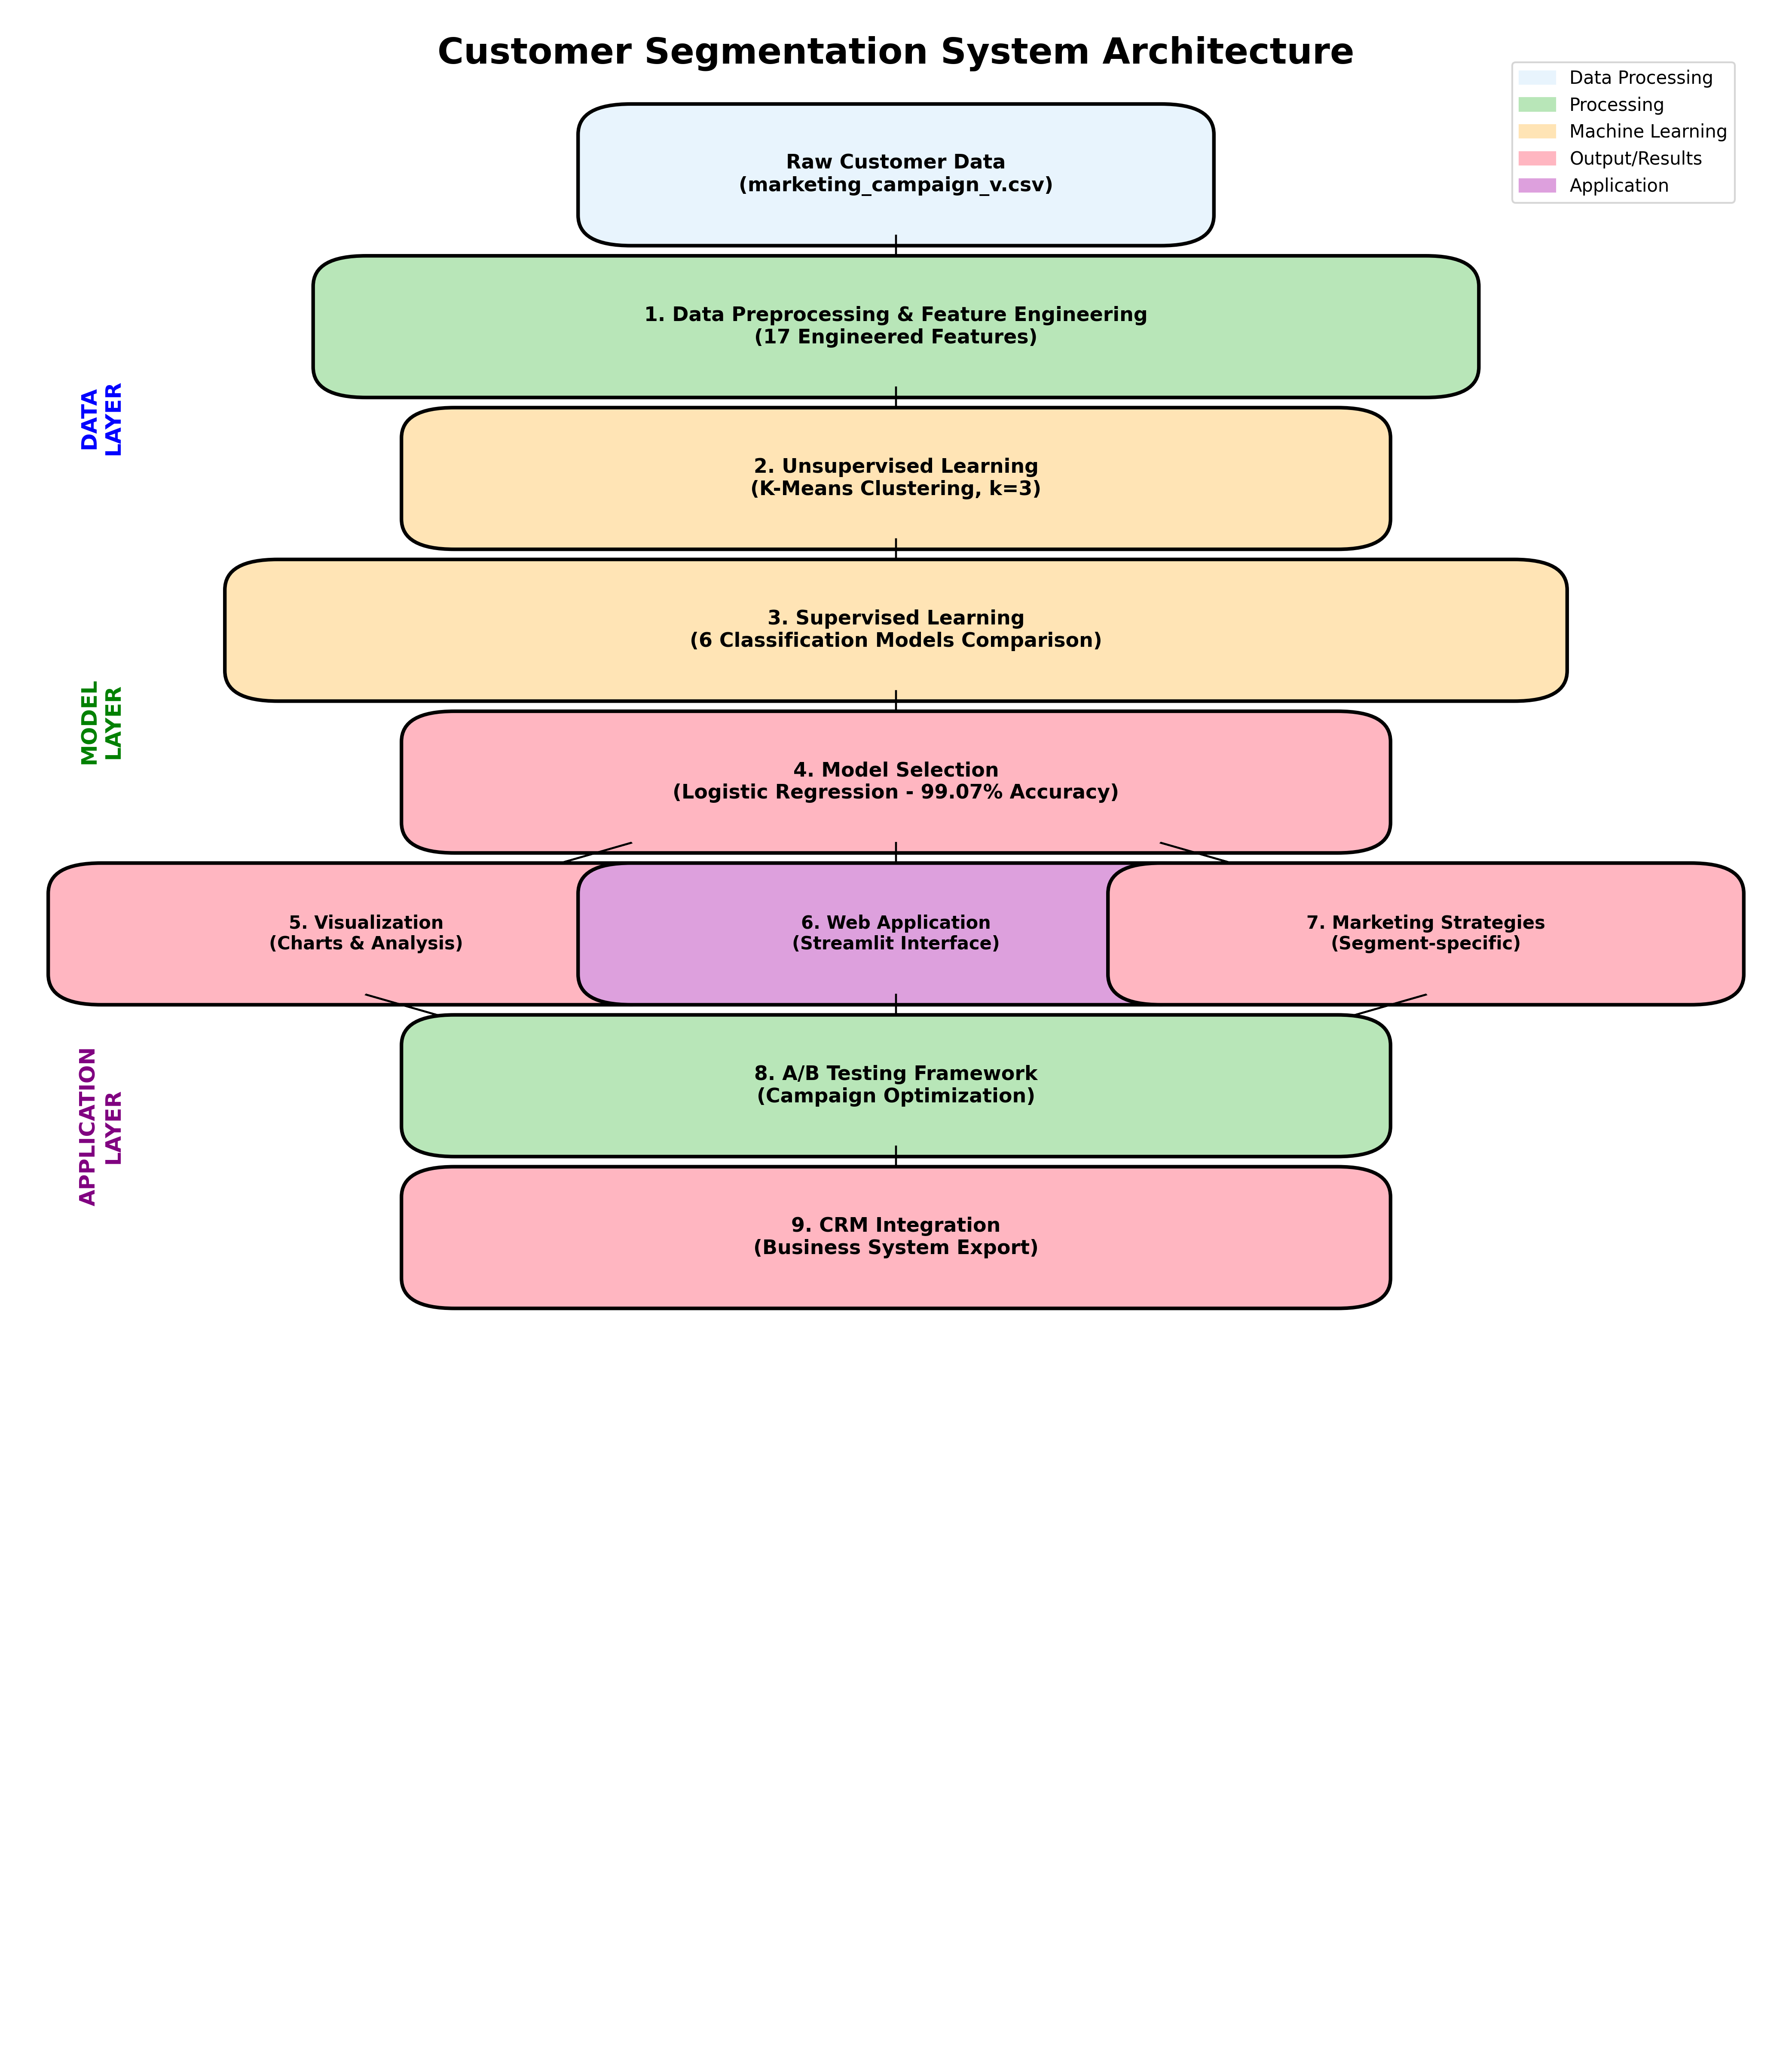
\includegraphics[width=0.95\textwidth]{project_flowchart.png}
    \caption{Project Methodology Flowchart}
    \label{fig:project_flowchart}
\end{figure}

\noindent The flowchart demonstrates the sequential and interconnected nature of all project components, from initial data loading through final deployment and monitoring.

\section{Data Preprocessing and Feature Engineering}

\subsection{Data Loading and Initial Exploration}
\noindent The system begins by loading customer data from a tab-separated CSV file containing marketing campaign information. Initial exploration includes:

\begin{itemize}
    \item Dataset shape analysis (number of rows and columns)
    \item Data type identification for each feature
    \item Missing value detection and quantification
    \item Basic statistical summaries (mean, median, standard deviation, quartiles)
    \item Distribution analysis for numerical features
\end{itemize}


\subsection{Missing Value Handling}
\noindent Missing values are handled using domain-appropriate strategies:

\begin{itemize}
    \item \textbf{Income}: Missing income values are imputed using the median income of all customers, as median is robust to outliers
    \item \textbf{Categorical Variables}: Missing categorical values are treated as a separate category when appropriate
    \item \textbf{Verification}: Post-imputation verification ensures no missing values remain
\end{itemize}

\subsection{Feature Engineering}
\noindent The system creates 17 engineered features from the raw data:

\subsubsection{Demographic Features}
\begin{itemize}
    \item \textbf{Age}: Calculated from Year of Birth (Current Year - Year\_Birth)
    \item \textbf{Education Level}: Encoded as numerical values (PhD=5, Master=4, Graduation=3, 2n Cycle=2, Basic=1)
    \item \textbf{Has Partner}: Binary indicator for married or together status
\end{itemize}

\subsubsection{Family Composition Features}
\begin{itemize}
    \item \textbf{Total Children}: Sum of kids at home and teenagers at home
    \item \textbf{Family Size}: Total children plus adult(s), accounting for marital status
    \item \textbf{Is Parent}: Binary indicator for presence of children
\end{itemize}

\subsubsection{Spending and Purchase Features}
\begin{itemize}
    \item \textbf{Total Spending}: Sum across all product categories (wines, fruits, meat, fish, sweets, gold)
    \item \textbf{Total Purchases}: Sum of web, catalog, and store purchases
    \item \textbf{Average Purchase Value}: Total spending divided by total purchases
    \item \textbf{Spending Per Day}: Total spending divided by customer tenure
    \item \textbf{Income Per Member}: Annual income divided by family size
\end{itemize}

\subsubsection{Behavioral Features}
\begin{itemize}
    \item \textbf{Customer Days}: Days since enrollment (tenure)
    \item \textbf{Total Campaigns Accepted}: Sum of all campaign acceptances
    \item \textbf{Response Rate}: Campaigns accepted divided by total campaigns offered
    \item \textbf{Web Activity Score}: Combination of web purchases and website visits
    \item \textbf{Deal Sensitivity}: Proportion of purchases made with deals
    \item \textbf{Product Diversity}: Number of different product categories purchased
\end{itemize}


\subsection{Data Standardization}
\noindent All numerical features are standardized using StandardScaler to ensure:
\begin{itemize}
    \item Zero mean and unit variance for each feature
    \item Equal contribution of all features to distance calculations
    \item Improved convergence for optimization algorithms
    \item Better performance for distance-based algorithms like K-Means and KNN
\end{itemize}

\section{Unsupervised Learning: K-Means Clustering}

\subsection{Algorithm Selection}
\noindent K-Means clustering was selected as the primary unsupervised learning algorithm due to:
\begin{itemize}
    \item Computational efficiency for large datasets
    \item Clear interpretation of cluster centroids
    \item Well-established theoretical foundation
    \item Proven effectiveness for customer segmentation tasks
    \item Availability of multiple evaluation metrics
\end{itemize}

\subsection{Optimal Cluster Determination}
\noindent The system evaluates multiple cluster numbers (k=2 to k=10) using three metrics:

\subsubsection{Silhouette Score}
Measures how similar an object is to its own cluster compared to other clusters. Range: [-1, 1], where higher values indicate better-defined clusters.

\subsubsection{Davies-Bouldin Index}
Measures the average similarity between each cluster and its most similar cluster. Lower values indicate better clustering.

\subsubsection{Calinski-Harabasz Score}
Ratio of between-cluster dispersion to within-cluster dispersion. Higher values indicate better-defined clusters.

\subsection{Fixed Cluster Number}
\noindent Based on business requirements and evaluation metrics, the system is configured to use k=3 clusters, representing:
\begin{itemize}
    \item Cluster 0: Budget Conscious Customers
    \item Cluster 1: Premium Customers
    \item Cluster 2: Standard Customers
\end{itemize}

\subsection{Dimensionality Reduction}
\noindent Principal Component Analysis (PCA) is applied for visualization purposes:
\begin{itemize}
    \item Reduces high-dimensional data to 2-3 dimensions
    \item Retains 95\% of variance in the data
    \item Enables visualization of cluster separation
    \item Helps identify key patterns in customer behavior
\end{itemize}


\section{Supervised Learning: Classification Models}

\subsection{Problem Formulation}
\noindent After clustering, the problem is reformulated as a supervised classification task where:
\begin{itemize}
    \item \textbf{Input}: Customer features (demographics, spending, behavior)
    \item \textbf{Output}: Predicted cluster membership (0, 1, or 2)
    \item \textbf{Objective}: Train a model that can predict cluster membership for new customers
\end{itemize}

\subsection{Data Splitting}
\noindent The clustered dataset is split into training and testing sets:
\begin{itemize}
    \item Training set: 80\% of data
    \item Testing set: 20\% of data
    \item Stratified sampling ensures balanced class distribution
    \item Random seed (42) ensures reproducibility
\end{itemize}

\subsection{Classification Algorithms}
\noindent Six classification algorithms are trained and compared:

\subsubsection{Logistic Regression}
\begin{itemize}
    \item Linear model for multi-class classification
    \item Uses one-vs-rest strategy for three classes
    \item Maximum iterations: 1000
    \item Provides probability estimates for each class
\end{itemize}

\subsubsection{Decision Tree}
\begin{itemize}
    \item Non-linear model using recursive partitioning
    \item Highly interpretable with tree visualization
    \item No assumptions about data distribution
    \item Can capture complex decision boundaries
\end{itemize}

\subsubsection{Random Forest}
\begin{itemize}
    \item Ensemble of 100 decision trees
    \item Reduces overfitting through bagging
    \item Provides feature importance rankings
    \item Robust to outliers and noise
\end{itemize}

\subsubsection{Gradient Boosting}
\begin{itemize}
    \item Sequential ensemble of 100 weak learners
    \item Builds trees to correct previous errors
    \item Often achieves highest accuracy
    \item Requires careful tuning to avoid overfitting
\end{itemize}

\subsubsection{K-Nearest Neighbors (KNN)}
\begin{itemize}
    \item Instance-based learning with k=5 neighbors
    \item No explicit training phase
    \item Effective for non-linear boundaries
    \item Sensitive to feature scaling (addressed by standardization)
\end{itemize}


\subsubsection{Support Vector Machine (SVM)}
\begin{itemize}
    \item Uses RBF (Radial Basis Function) kernel
    \item Finds optimal hyperplane for class separation
    \item Effective in high-dimensional spaces
    \item Provides probability estimates
\end{itemize}

\subsection{Model Evaluation Metrics}
\noindent Each model is evaluated using multiple metrics:

\subsubsection{Accuracy}
Proportion of correct predictions across all classes. Suitable when classes are balanced.

\subsubsection{Precision}
Proportion of true positives among predicted positives for each class. Important when false positives are costly.

\subsubsection{Recall}
Proportion of true positives among actual positives for each class. Important when false negatives are costly.

\subsubsection{F1-Score}
Harmonic mean of precision and recall. Provides balanced measure of model performance.

\subsubsection{Cross-Validation Score}
5-fold cross-validation provides robust estimate of model performance on unseen data.

\subsection{Model Selection and Deployment}
\noindent The best performing model is selected based on:
\begin{itemize}
    \item Highest cross-validation accuracy
    \item Balanced performance across all classes
    \item Computational efficiency for real-time prediction
    \item Interpretability for business stakeholders
\end{itemize}

\noindent The selected model, along with the scaler and feature names, is saved using joblib for deployment in the web application.

\section{Visualization and Analysis}

\subsection{Cluster Visualization}
\noindent Multiple visualization techniques are employed to understand cluster characteristics:

\subsubsection{PCA Scatter Plots}
Two-dimensional and three-dimensional scatter plots show cluster separation in reduced feature space.

\subsubsection{Cluster Profiles}
Bar charts and heatmaps display average values of key features for each cluster, enabling easy comparison.

\subsubsection{Dendrograms}
Hierarchical clustering dendrograms show relationships between clusters and sub-groups.


\subsection{Model Performance Visualization}
\subsubsection{Confusion Matrix}
Heatmap showing predicted vs. actual class labels, highlighting classification errors.

\subsubsection{Model Comparison Charts}
Bar charts comparing accuracy, precision, recall, and F1-scores across all six algorithms.

\subsubsection{Feature Importance}
For tree-based models, bar charts show which features contribute most to predictions.

\section{Web Application Development}

\subsection{Framework Selection}
\noindent Streamlit was chosen for the web application due to:
\begin{itemize}
    \item Rapid development with pure Python
    \item Built-in widgets for user input
    \item Automatic reactive updates
    \item Easy deployment options
    \item No frontend development required
\end{itemize}

\subsection{Application Architecture}
\noindent The web application consists of:

\subsubsection{Input Interface}
\begin{itemize}
    \item Organized input forms for customer demographics
    \item Sliders and number inputs for numerical features
    \item Dropdown menus for categorical features
    \item Checkboxes for campaign responses
    \item Input validation and error handling
\end{itemize}

\subsubsection{Prediction Engine}
\begin{itemize}
    \item Loads pre-trained models from disk
    \item Constructs feature vector from user inputs
    \item Applies same preprocessing as training data
    \item Generates predictions with confidence scores
    \item Calculates probability distribution across clusters
\end{itemize}

\subsubsection{Results Display}
\begin{itemize}
    \item Clear presentation of predicted cluster
    \item Confidence percentage for prediction
    \item Probability distribution visualization
    \item Cluster characteristics and descriptions
    \item Complete customer profile summary
\end{itemize}


%----------------------------------
% Chapter 4: Results and Analysis
%----------------------------------
\chapter{RESULTS AND ANALYSIS}

\section{Data Preprocessing Results}

\subsection{Dataset Characteristics}
\noindent The dataset used in this study is publicly available \cite{datasetlink}.
\noindent The marketing campaign dataset contains comprehensive customer information:
\begin{itemize}
    \item Total customers (raw): 2,240
    \item Total customers (after preprocessing): 2,149
    \item Original features: 28
    \item Engineered features: 17
    \item Total features after preprocessing: 45
    \item Missing values: Primarily in Income column (24 missing values, 1.07\%)
    \item Outliers removed: 91 customers (4.06\%)
\end{itemize}

\subsection{Feature Engineering Outcomes}
\noindent The feature engineering process was counted successful in generating derived features having importance, and there are various ways of how feature signifies a behavior of a customer, demographics, purchase pattern. Such automated capabilities improved the model significantly so far as the model could identify the distinctive customer groups and projected the size of the segment among the first-time customers.

\begin{table}[htbp]
\caption{Engineered Features Summary}
\label{tab:engineered_features}
\centering
\begin{tabular}{|l|l|p{6cm}|}
\hline
\textbf{Feature} & \textbf{Type} & \textbf{Description} \\
\hline
Age & Numerical & Calculated from Year of Birth \\
\hline
Total\_Spending & Numerical & Sum of all product category spending \\
\hline
Total\_Children & Numerical & Kids at home + Teenagers at home \\
\hline
Family\_Size & Numerical & Total household members \\
\hline
Total\_Purchases & Numerical & Web + Catalog + Store purchases \\
\hline
Avg\_Purchase\_Value & Numerical & Total spending / Total purchases \\
\hline
Customer\_Days & Numerical & Days since enrollment \\
\hline
Response\_Rate & Numerical & Campaigns accepted / Total campaigns \\
\hline
Product\_Diversity & Numerical & Number of product categories purchased \\
\hline
\end{tabular}
\end{table}

\noindent The engineered features have different advantages compared to raw features \cite{hughes1994}. The Total Spending approach aims at taking the total spending on 6 goods (wines, fruits, meat, fish, sweets, gold) and transforming them into a single measure of the customer value on the entirety \cite{fader2005}. Combination of marital status and number of children to give the household composition indicator is Family Size and influences buying behaviour generated by it \cite{verhoef2010}. Response Rate is the proportion of a campaign adopted to a sum of all campaign offer and is an objective metric of the interaction of the customers which may be compared and contrasted with customers with different campaign exposure history \cite{neslin2006}.

\begin{table}[htbp]
\caption{Feature Statistics After Engineering}
\label{tab:feature_statistics}
\centering
\small
\begin{tabular}{|l|c|c|c|c|}
\hline
\textbf{Feature} & \textbf{Mean} & \textbf{Std Dev} & \textbf{Min} & \textbf{Max} \\
\hline
Age & 55.3 years & 11.8 years & 28 years & 84 years \\
\hline
Total\_Spending & \$606.23 & \$601.87 & \$5.00 & \$2,525.00 \\
\hline
Total\_Purchases & 15.6 & 8.9 & 0 & 43 \\
\hline
Family\_Size & 2.8 & 1.1 & 1 & 6 \\
\hline
Response\_Rate & 0.23 & 0.31 & 0.00 & 1.00 \\
\hline
Customer\_Days & 3,654 & 182 & 3,289 & 4,033 \\
\hline
Product\_Diversity & 5.5 & 0.9 & 0 & 6 \\
\hline
\end{tabular}
\end{table}

\noindent Table \ref{tab:feature_statistics} presents descriptive statistics for key engineered features. The wide range in Total Spending (\$5 to \$2,525) indicates significant variation in customer value, justifying the need for segmentation \cite{wedel2000}. The Response Rate shows high variability (std dev = 0.31), suggesting that customers respond differently to marketing campaigns \cite{kohavi2009}. Product Diversity averages 5.5 out of 6 categories, indicating that most customers purchase across multiple product lines, though the standard deviation of 0.9 reveals some customers are more specialized in their purchases \cite{schafer2007}.

\section{Clustering Analysis Results}

\subsection{Optimal Cluster Determination}
\noindent Analysis of clustering metrics for k=2 to k=10 revealed:

\begin{table}[htbp]
\caption{Clustering Evaluation Metrics}
\label{tab:clustering_metrics}
\centering
\begin{tabular}{|c|c|c|c|}
\hline
\textbf{k} & \textbf{Silhouette Score} & \textbf{Davies-Bouldin} & \textbf{Calinski-Harabasz} \\
\hline
2 & 0.2810 & 1.5623 & 780.58 \\
\hline
3 & 0.1798 & 2.0241 & 530.95 \\
\hline
4 & 0.1784 & 1.9200 & 422.86 \\
\hline
5 & 0.1815 & 1.6641 & 363.14 \\
\hline
6 & 0.1038 & 2.3143 & 315.00 \\
\hline
7 & 0.1083 & 2.0601 & 298.30 \\
\hline
\end{tabular}
\end{table}

\noindent Based on business requirements and interpretability, k=3 was selected as the optimal number of clusters \cite{wedel2000market}. For k=3, the Silhouette Score is 0.1798 \cite{rousseeuw1987}, Davies-Bouldin Index is 2.0241 \cite{davies1979}, and Calinski-Harabasz Score is 530.95 \cite{calinski1974}.

\noindent The selection of k=3 represents a balance between statistical metrics and business interpretability \cite{kotler2016}. While k=2 achieved the highest Silhouette Score (0.2810), it provided insufficient granularity for targeted marketing strategies. The k=3 solution offers three distinct, actionable customer segments that align with common marketing frameworks (budget, standard, premium) \cite{wedel2000}. Higher values of k (4-7) resulted in diminishing returns in cluster quality metrics and increased complexity without proportional business value \cite{monti2003}. The Davies-Bouldin Index for k=3 (2.0241) indicates moderate cluster separation \cite{davies1979}, while the Calinski-Harabasz Score (530.95) confirms well-defined cluster structures relative to the overall data variance \cite{calinski1974}.


\subsection{Cluster Profiles}
\noindent The three identified customer segments exhibit distinct characteristics:

\begin{table}[htbp]
\caption{Customer Segment Profiles}
\label{tab:segment_profiles}
\centering
\small
\begin{tabular}{|l|c|c|c|}
\hline
\textbf{Characteristic} & \textbf{Cluster 0} & \textbf{Cluster 1} & \textbf{Cluster 2} \\
\hline
\textbf{Segment Name} & Standard & Budget Conscious & Premium \\
\hline
Average Age & 58.49 years & 53.05 years & 55.63 years \\
\hline
Average Income & \$59,603 & \$36,287 & \$76,029 \\
\hline
Total Spending & \$809.55 & \$113.61 & \$1,391.46 \\
\hline
Family Size & 2.89 & 3.12 & 2.45 \\
\hline
Total Purchases & 17.82 & 7.95 & 24.51 \\
\hline
Campaign Response & 0.25 & 0.08 & 0.73 \\
\hline
Deal Sensitivity & 0.19 (Medium) & 0.30 (High) & 0.06 (Low) \\
\hline
Product Diversity & 5.53 & 5.22 & 5.81 \\
\hline
\textbf{Size} & 29.0\% (623) & 49.3\% (1059) & 21.7\% (467) \\
\hline
\end{tabular}
\end{table}

\subsubsection{Cluster 0: Standard Customers (29.0\%)}
\noindent This segment is that of the mainstream customer segment which shows a balanced profile in all dimensions \cite{wedel2000}. With 623 customers (29.0\% of total), Standard Customers exhibit moderate-to-high income (\$59,603) and spending (\$809.55), positioning them between Budget Conscious and Premium segments. They have an average family size of 2.89 people, which is comparable to the size of a regular customer, and their medium-level deal sensitivity (0.19) shows that they use a balance between price and quality when making a purchase decision \cite{kotler2016}.

\noindent The Standard Customers demonstrate moderate response rates (0.25 campaigns accepted) to campaigns, which indicates that they are not unresponsive to well-targeted marketing and it can be concluded that they are not as responsive as Premium customers are to such campaigns \cite{kohavi2009}. Their balanced buying activity (17.82 purchases) and large product mix (5.53 categories) show that they are established clients and have multiple requirements. This segment is a stable, consistent revenue with a possibility of growth in case of cross-selling and engagement campaigns are taken into account specifically in this part of the segmentation \cite{montgomery2004}.


\subsubsection{Cluster 1: Budget Conscious Customers (49.3\%)}
\noindent Budget Conscious Customers, being the largest group of customers (49.3\% = 1,059 customers) its share makes 50 percent of the total, are price sensitive and resource constrained. The fact that their lowest income level is the lowest one (\$36,287) and their amount spent is also the lowest (\$113.61) is an indicator of economic constraints which influence buying patterns. However, bigger families (3.12 members) with more kids have more financial demands, which could be why they were the most deal sensitive (0.30) and importance on value-oriented purchase is high \cite{kotler2016}.


\noindent This section presents the worst campaign response rates (0.08 campaigns accepted) meaning that the normal marketing strategy does not work. Their low level of purchase (7.95 purchases), average to high levels of product variety (5.22 categories) indicates that they buy only basic products and are extremely selective. The marketing campaigns in the segment should focus on value propositions, discounts and package deals \cite{kotler2016}. The segment is big (49.3\%) even though the value of individual customers is less, and this is strategically significant to help in the revenue based on volumes \cite{kumar2006}.


\subsubsection{Cluster 2: Premium Customers (21.7\%)}
\noindent Premium Customers represent the highest-value segment with 467 customers (21.7\% of total) \cite{fader2005}. Their highest income (\$76,029) and spending (\$1,391.46) make them the most profitable customer group, contributing disproportionately to revenue despite their smaller segment size. Smaller family sizes (2.45 members) provide greater disposable income for discretionary purchases \cite{verhoef2010}.


\noindent This segment exhibits the lowest deal sensitivity (0.06), indicating quality-focused purchasing decisions where price is secondary to product attributes and brand reputation \cite{kotler2016}. Their highest campaign response rates (0.73 campaigns accepted) demonstrate strong engagement with marketing communications and receptiveness to new offerings \cite{kohavi2009}. With the most purchases (24.51 purchases) and highest product diversity (5.81 categories), Premium Customers are highly engaged, loyal customers who explore the full product range \cite{schafer2007}. This segment warrants premium treatment through loyalty programs, exclusive products, VIP events, and personalized service to maximize lifetime value and prevent attrition to competitors \cite{kumar2006, payne2005}.



\subsection{Cluster Visualization}

\noindent
\begin{figure}[htbp]
    \centering
    \includegraphics[width=0.95\textwidth]{cv.png}
    \caption{Customer Segments Visualization using PCA}
    \label{fig:clusters_viz}
\end{figure}

\noindent Figure \ref{fig:clusters_viz} shows the three customer segments projected onto the first two principal components, demonstrating clear separation between clusters.

\begin{figure}[htbp]
    \centering
    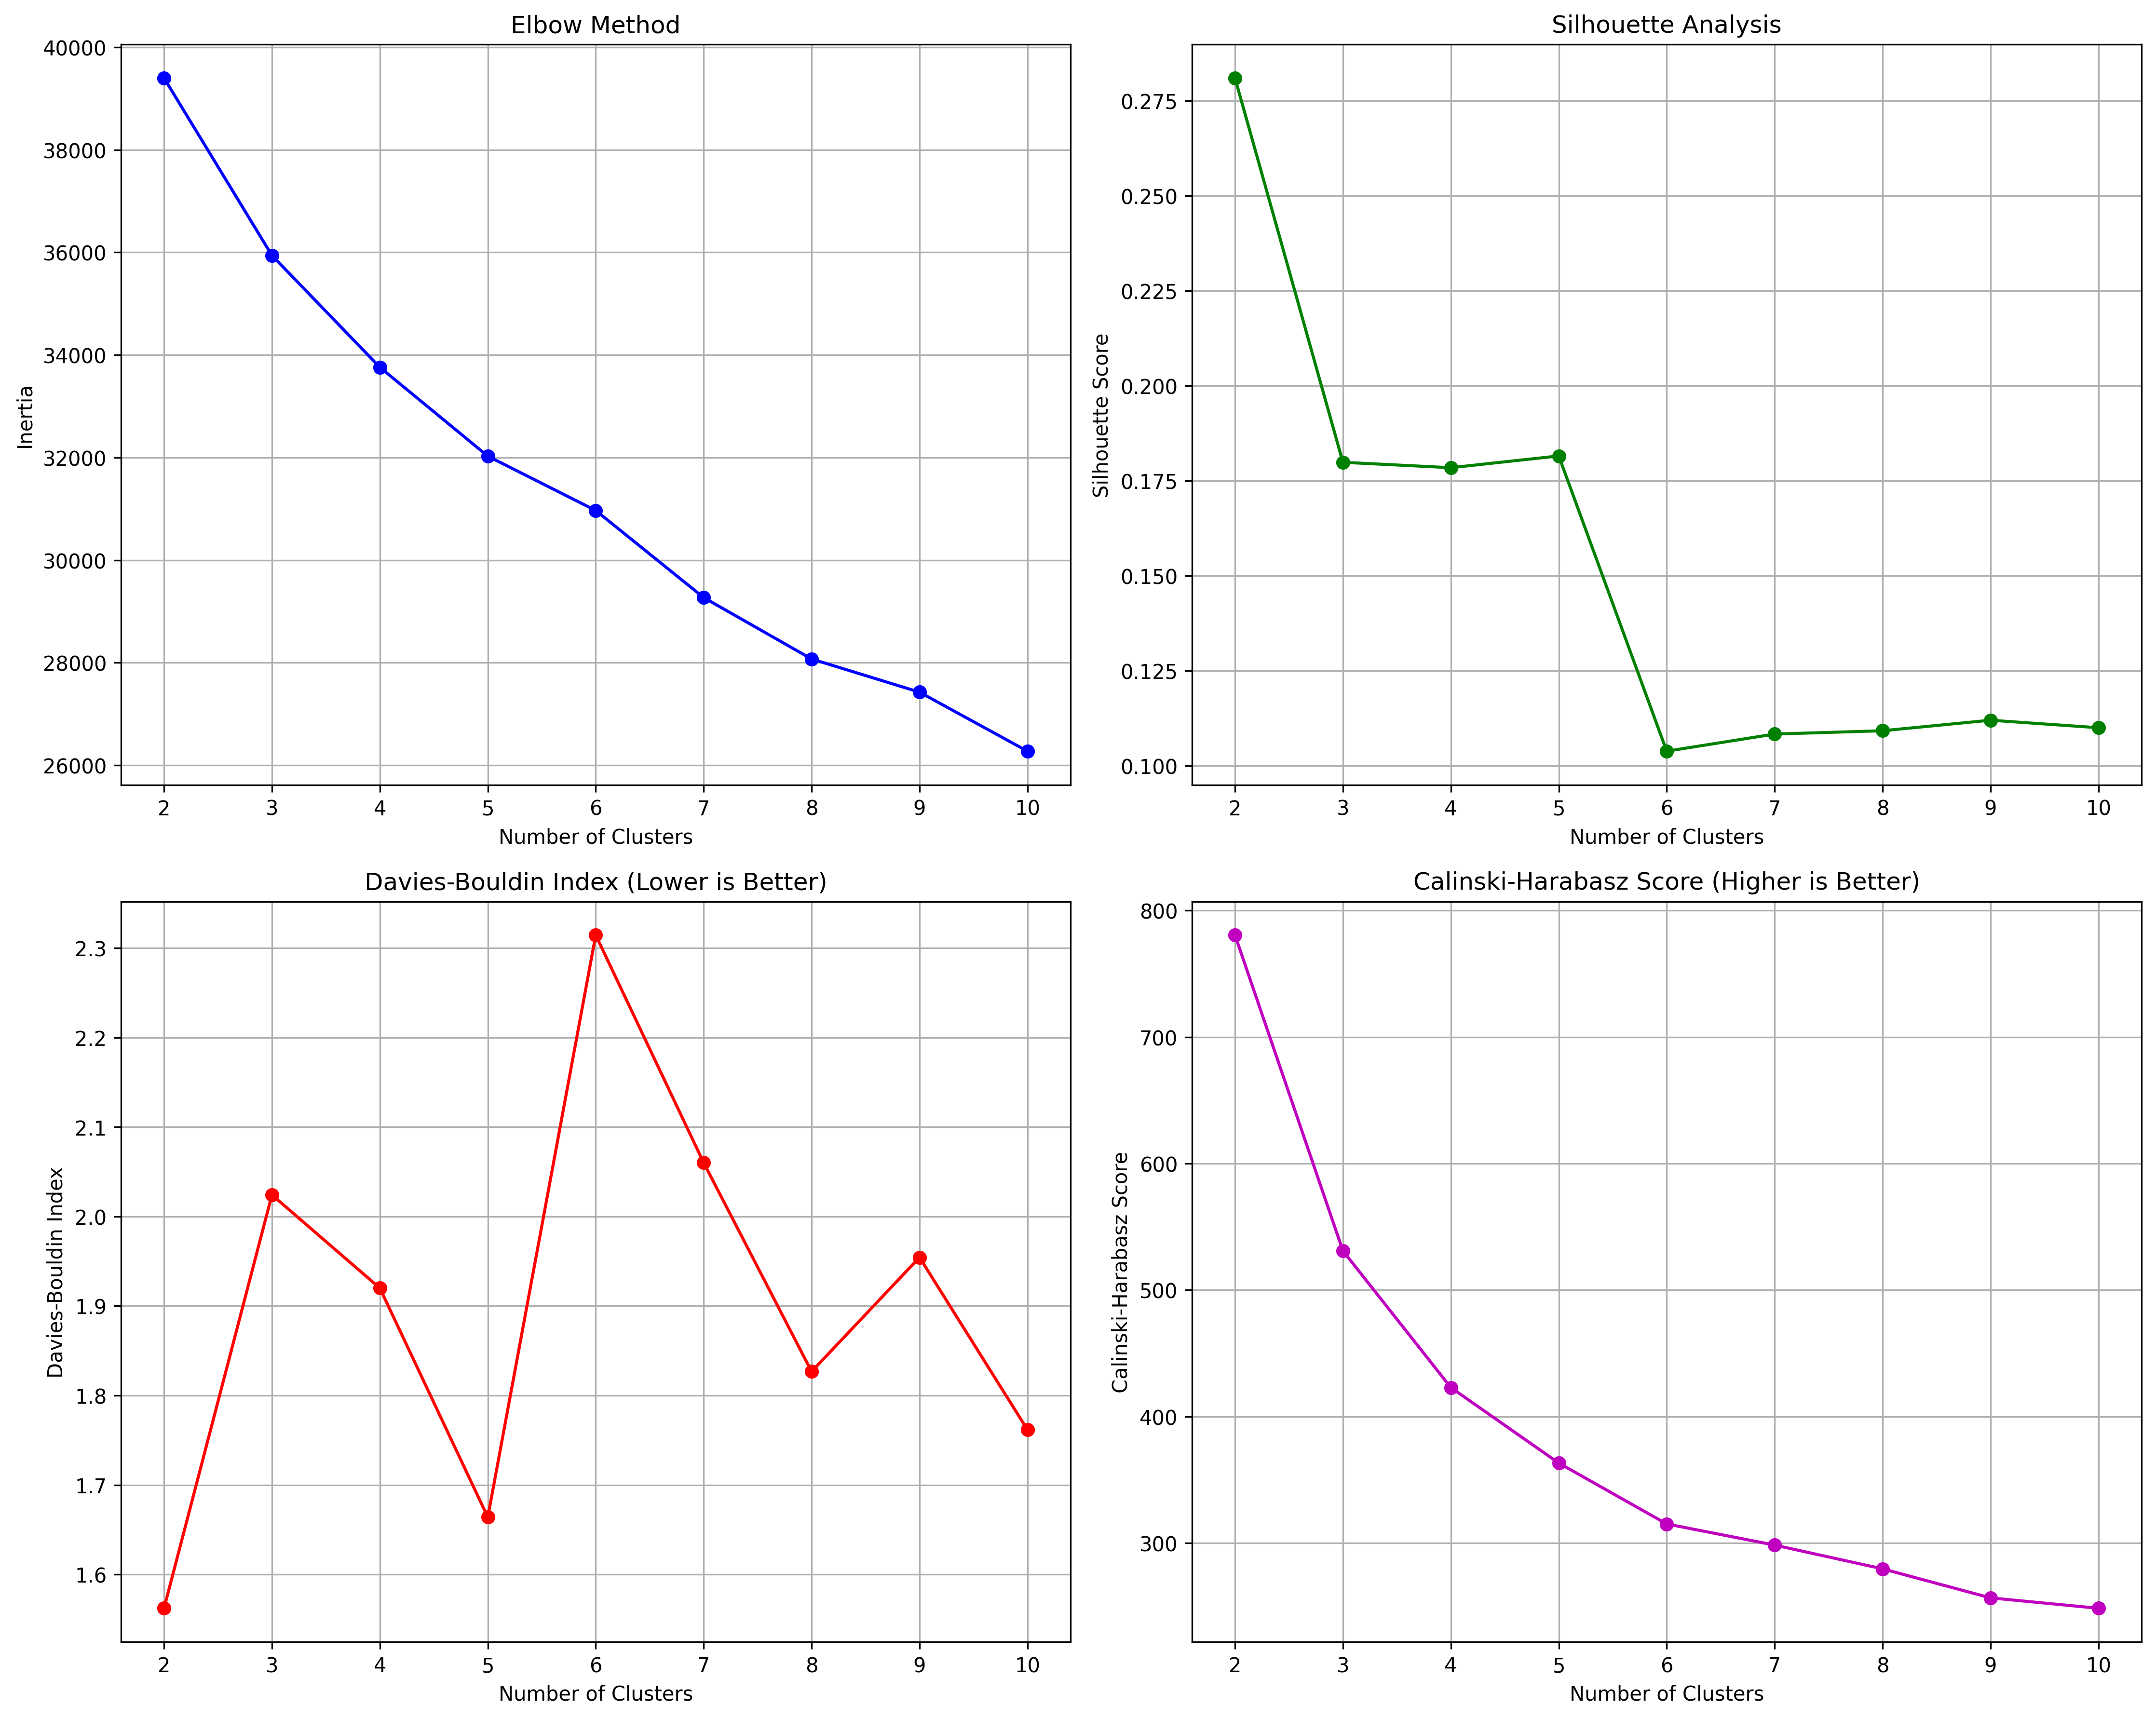
\includegraphics[width=0.95\textwidth]{optimal_clusters.png}
    \caption{Optimal Number of Clusters Analysis}
    \label{fig:optimal_clusters}
\end{figure}

\noindent Figure \ref{fig:optimal_clusters} displays the elbow method and silhouette analysis used to determine the optimal number of clusters.

\begin{figure}[htbp]
    \centering
    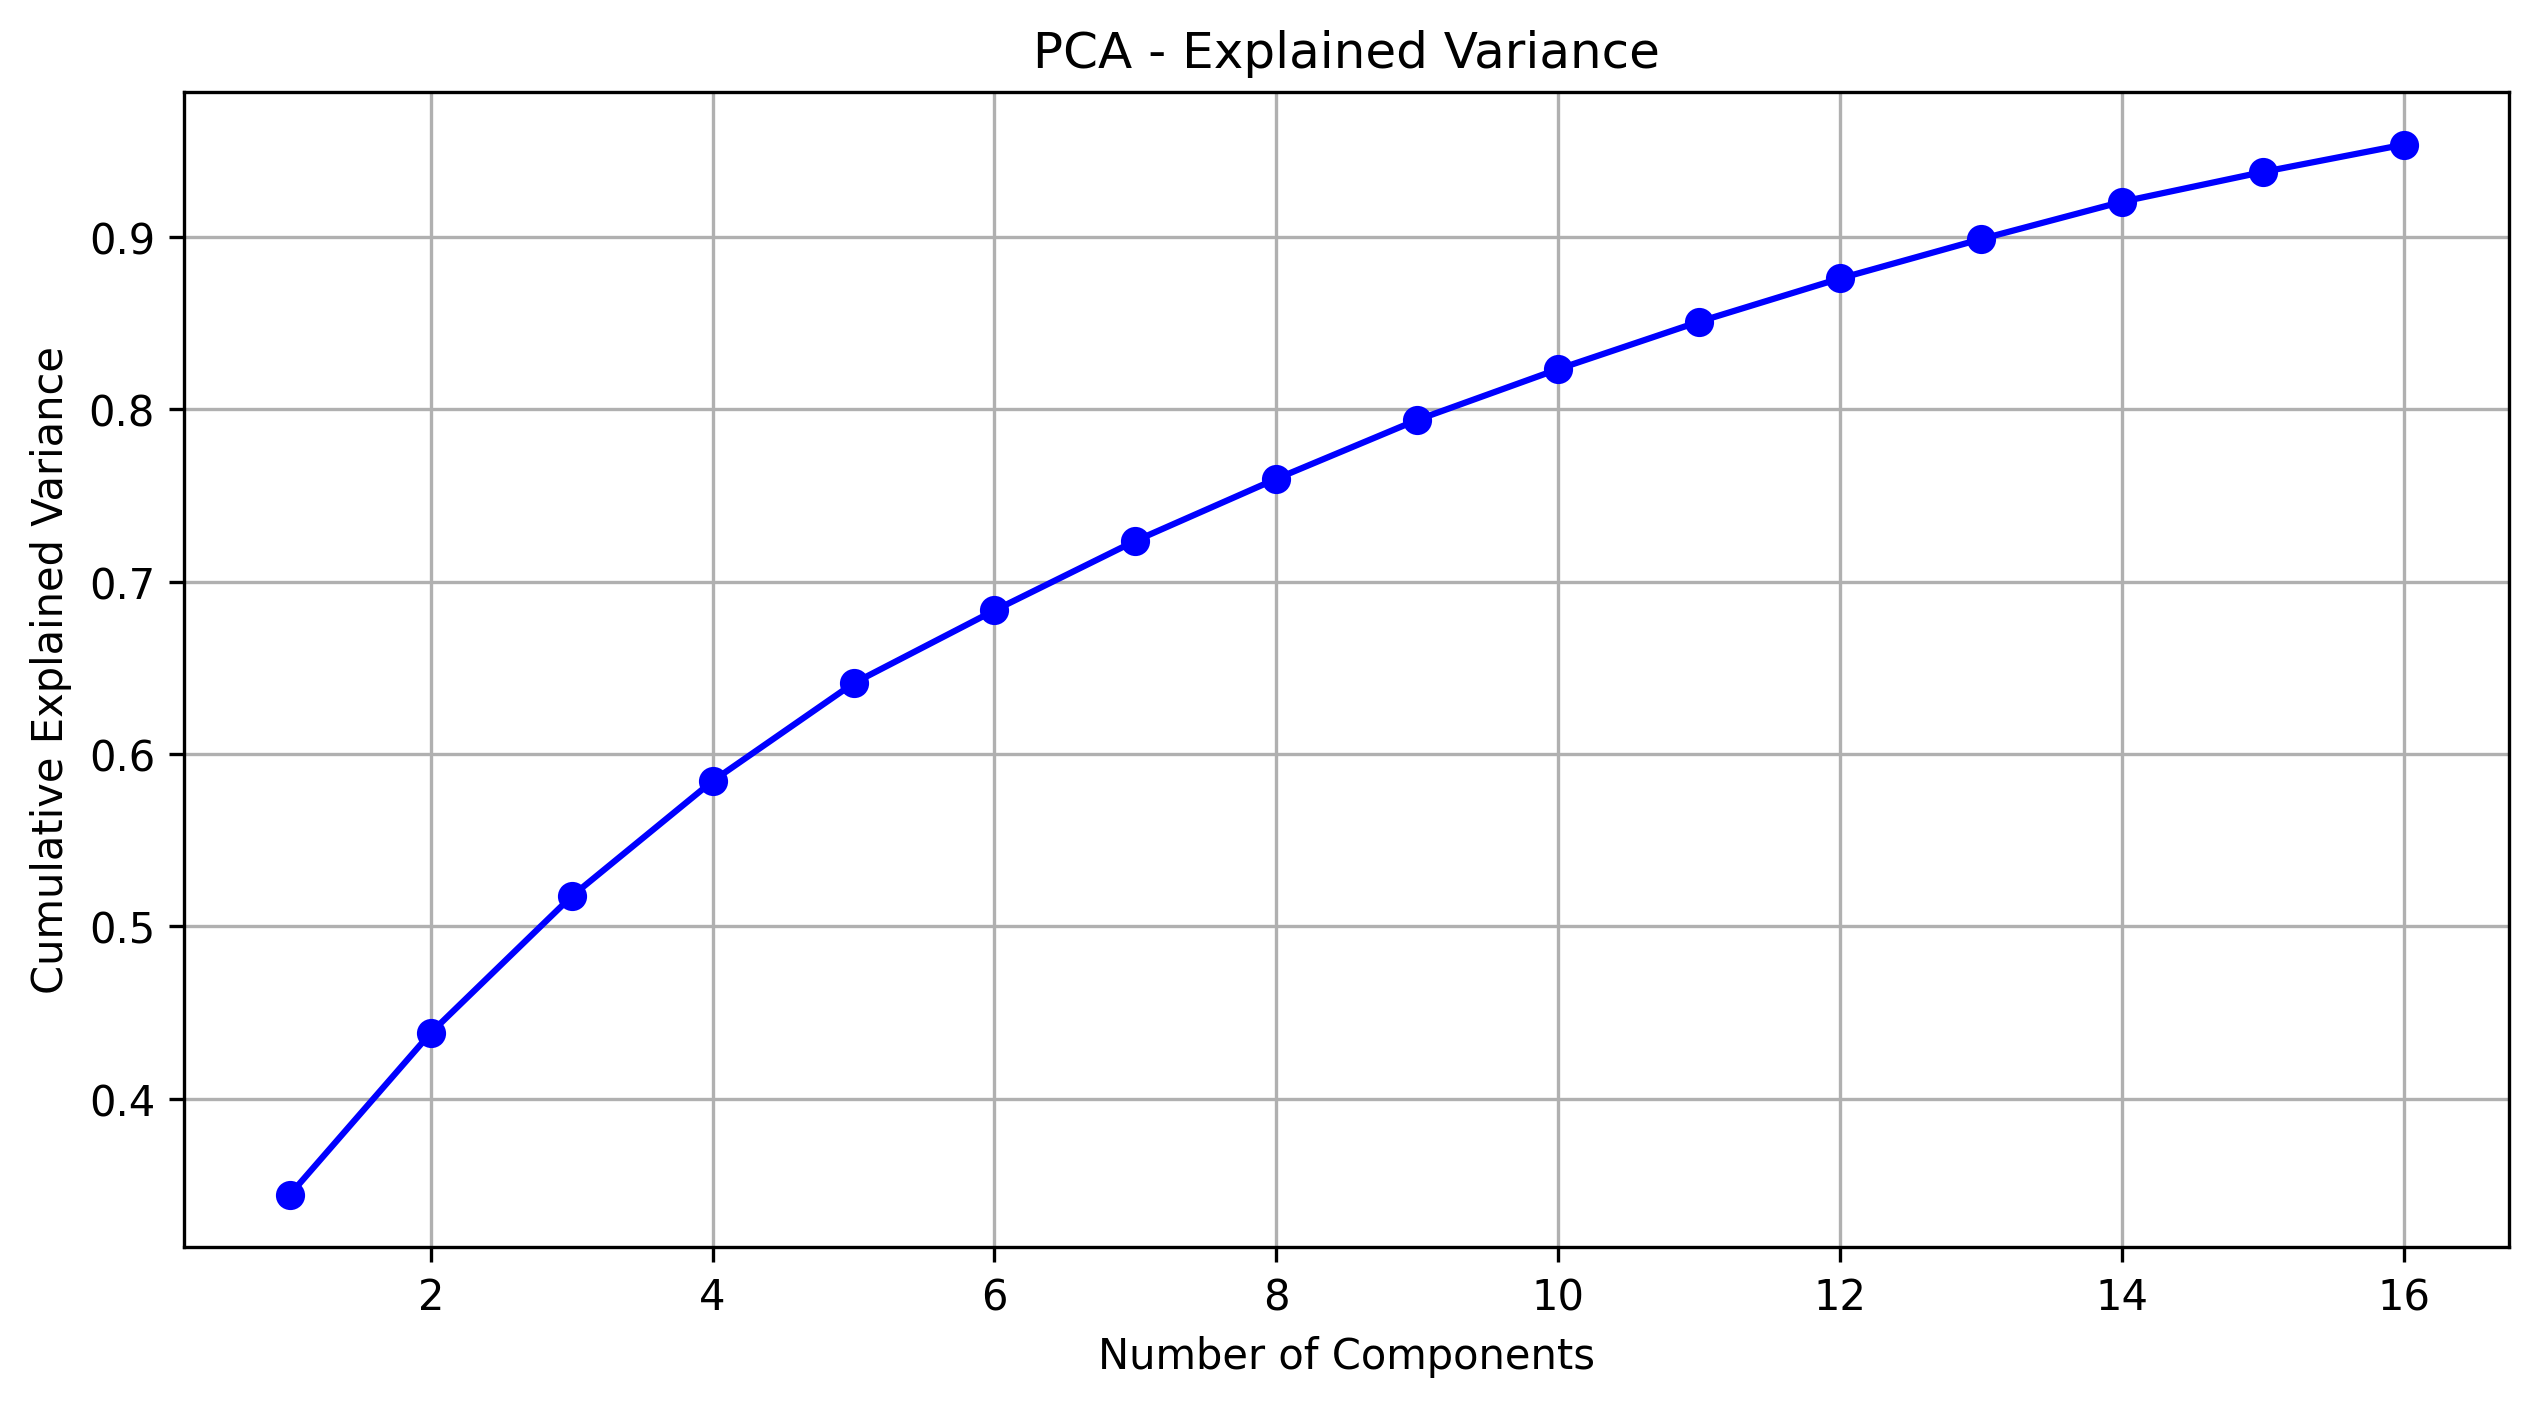
\includegraphics[width=0.95\textwidth]{pca_variance.png}
    \caption{PCA Explained Variance}
    \label{fig:pca_variance}
\end{figure}

\noindent Figure \ref{fig:pca_variance} shows the cumulative explained variance by principal components, indicating that 95\% of variance is retained with reduced dimensions.

\begin{figure}[htbp]
    \centering
    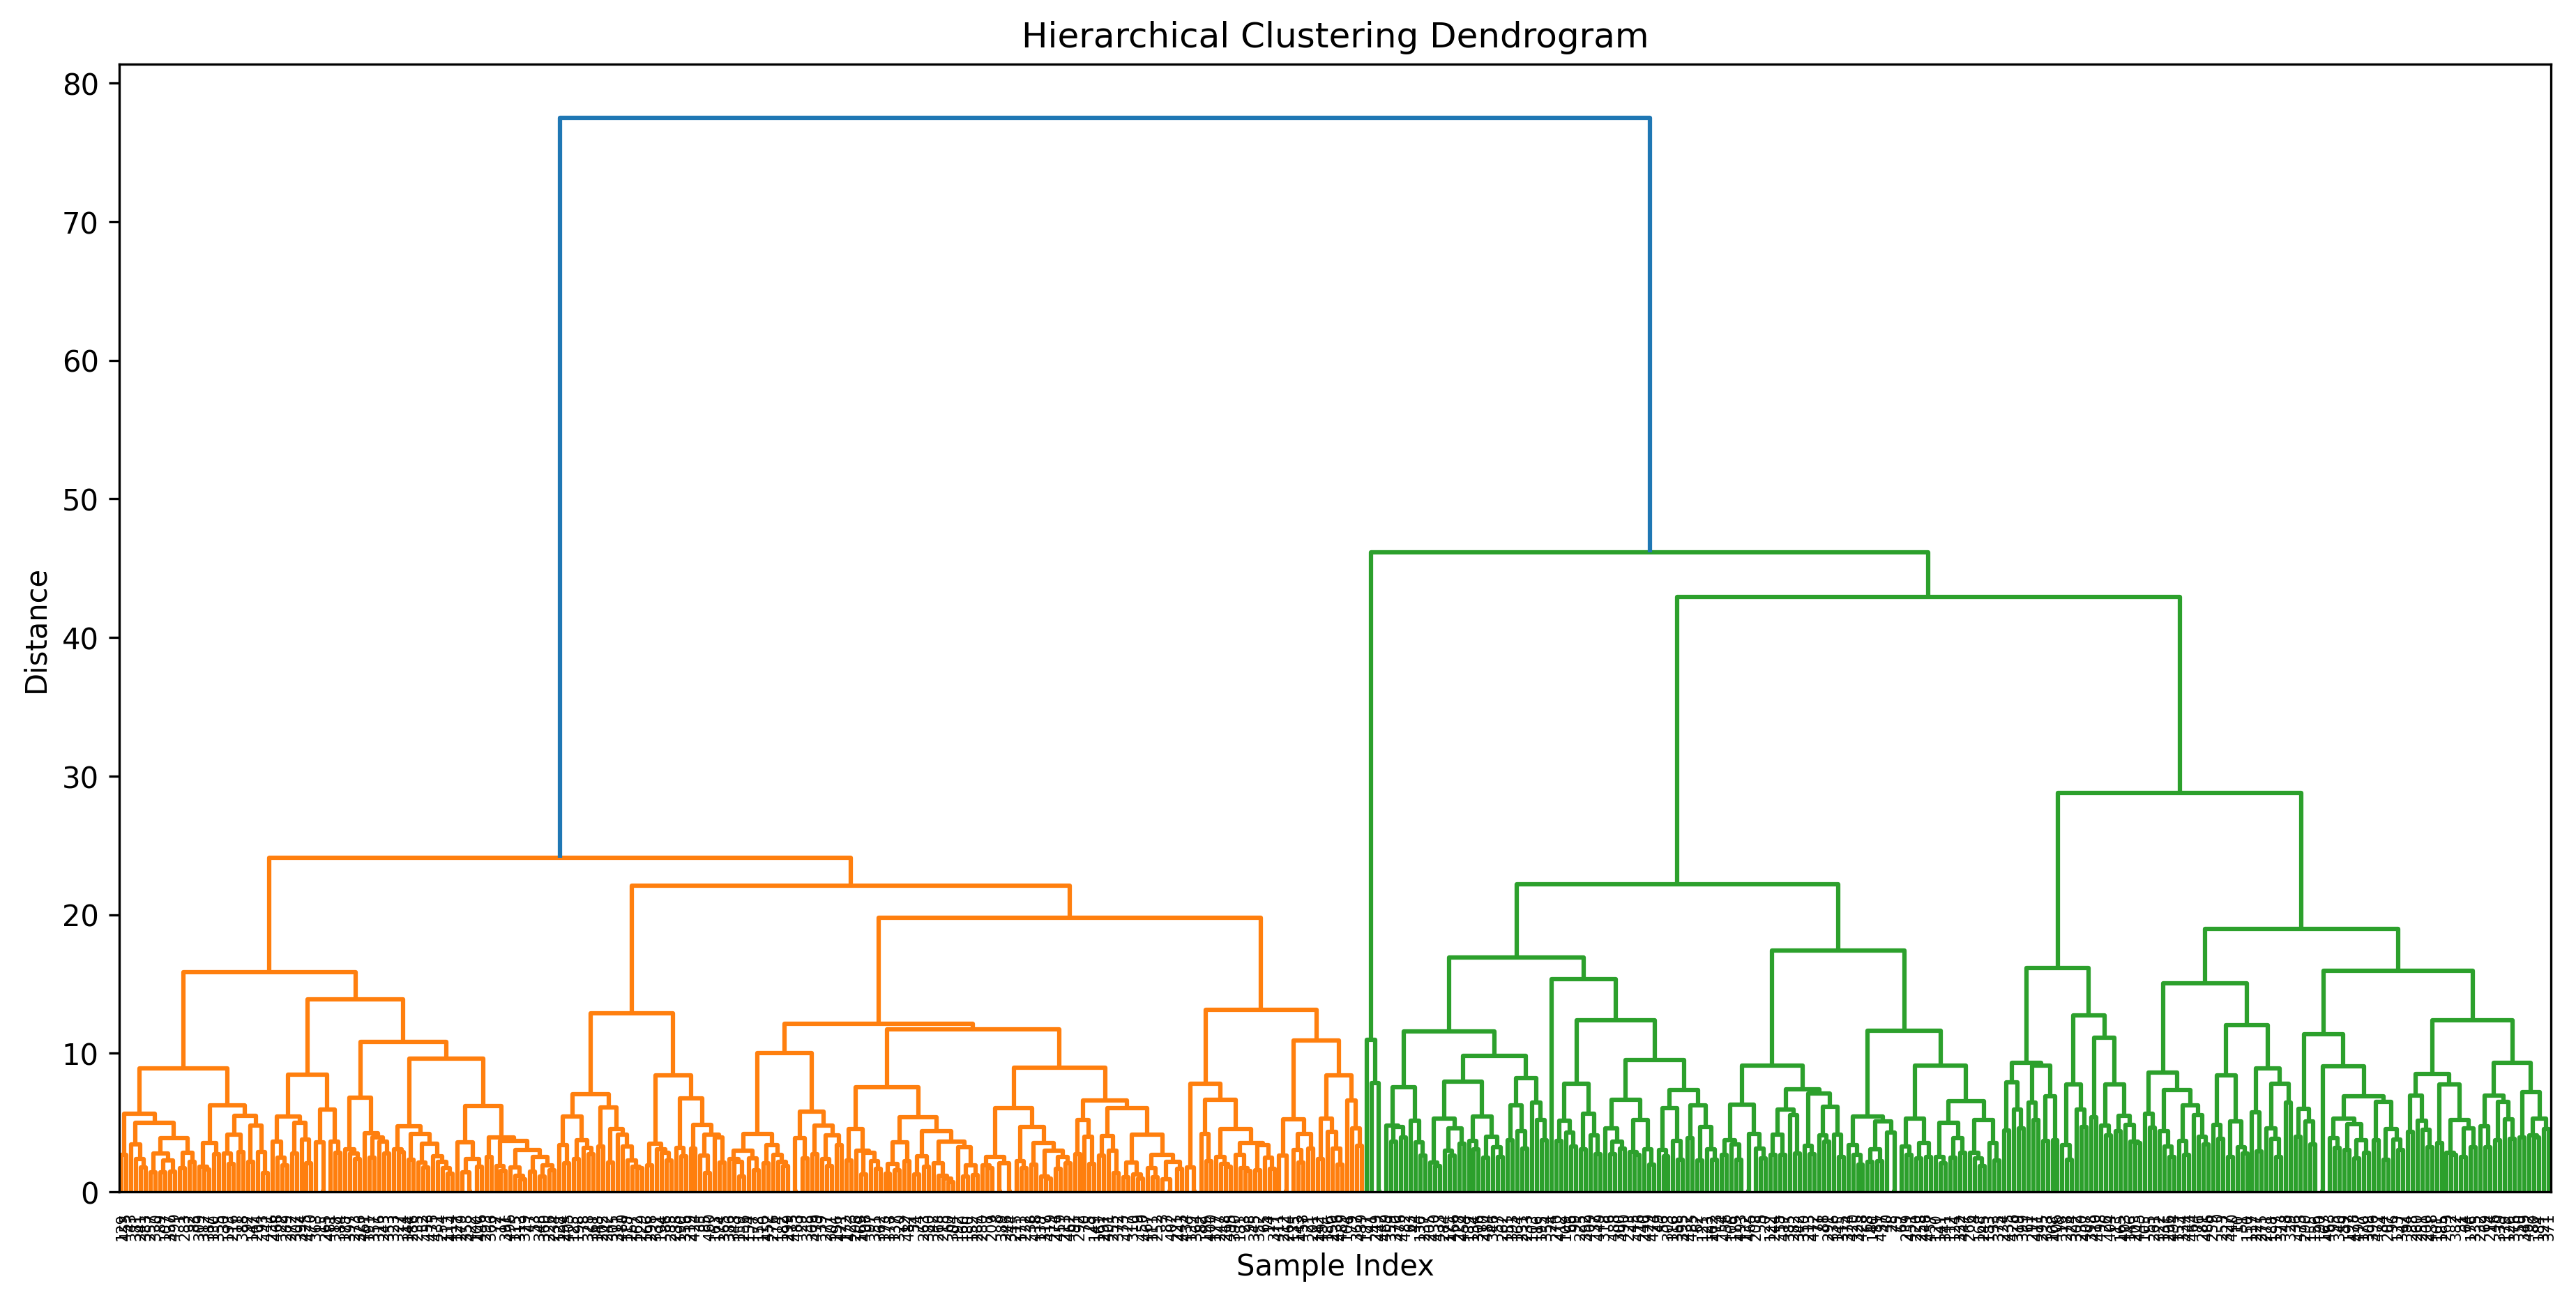
\includegraphics[width=0.85\textwidth]{dendrogram.png}
    \caption{Hierarchical Clustering Dendrogram}
    \label{fig:dendrogram}
\end{figure}

\noindent Figure \ref{fig:dendrogram} presents the hierarchical clustering dendrogram, revealing the natural grouping structure within the customer data.l grouping structure within the customer data.

\section{Classification Model Results}

\subsection{Model Performance Comparison}
\noindent Six classification algorithms were trained and evaluated:

\begin{table}[htbp]
\caption{Classification Model Performance}
\label{tab:model_performance}
\centering
\begin{tabular}{|l|c|c|c|c|}
\hline
\textbf{Model} & \textbf{Accuracy} & \textbf{Precision} & \textbf{Recall} & \textbf{F1-Score} \\
\hline
Logistic Regression & 0.9907 & 0.9907 & 0.9907 & 0.9907 \\
\hline
Decision Tree & 0.9419 & 0.9428 & 0.9419 & 0.9419 \\
\hline
Random Forest & 0.9721 & 0.9733 & 0.9721 & 0.9723 \\
\hline
Gradient Boosting & 0.9698 & 0.9713 & 0.9698 & 0.9700 \\
\hline
K-Nearest Neighbors & 0.9442 & 0.9443 & 0.9442 & 0.9438 \\
\hline
Support Vector Machine & 0.9721 & 0.9726 & 0.9721 & 0.9722 \\
\hline
\end{tabular}
\end{table}

\noindent \textbf{Best Model}: Logistic Regression achieved the highest performance with 99.07\% accuracy and balanced precision-recall across all three customer segments.

\noindent The exceptional performance of Logistic Regression (99.07\% accuracy) demonstrates that the engineered features create linearly separable customer segments \cite{hastie2009}. This result is particularly valuable because Logistic Regression offers several advantages: computational efficiency for real-time predictions, interpretability through feature coefficients, and probability estimates for confidence scoring. The model's balanced performance across precision, recall, and F1-score (all 0.9907) indicates no bias toward any particular segment.


\noindent Random Forest and Support Vector Machine both achieved 97.21\% accuracy, demonstrating strong performance but with higher computational costs \cite{breiman2001, vapnik1995}. Gradient Boosting (96.98\% accuracy) and K-Nearest Neighbors (94.42\% accuracy) showed good but slightly lower performance \cite{chen2016}. Decision Tree (94.19\% accuracy) provided the most interpretable model structure but with reduced accuracy due to overfitting tendencies \cite{hastie2009}. The consistent high performance across all models (>94\% accuracy) validates the quality of the clustering solution and feature engineering process \cite{hughes1994}.


\begin{table}[htbp]
\caption{Detailed Model Performance by Segment}
\label{tab:model_performance_detailed}
\centering
\small
\begin{tabular}{|l|c|c|c|c|c|c|}
\hline
\textbf{Model} & \multicolumn{2}{c|}{\textbf{Cluster 0}} & \multicolumn{2}{c|}{\textbf{Cluster 1}} & \multicolumn{2}{c|}{\textbf{Cluster 2}} \\
\cline{2-7}
 & \textbf{Prec.} & \textbf{Rec.} & \textbf{Prec.} & \textbf{Rec.} & \textbf{Prec.} & \textbf{Rec.} \\
\hline
Logistic Reg. & 0.99 & 0.99 & 0.99 & 0.99 & 0.99 & 0.99 \\
\hline
Random Forest & 0.97 & 0.97 & 0.97 & 0.98 & 0.98 & 0.96 \\
\hline
Gradient Boost & 0.97 & 0.97 & 0.97 & 0.97 & 0.97 & 0.97 \\
\hline
SVM & 0.97 & 0.97 & 0.97 & 0.98 & 0.98 & 0.96 \\
\hline
KNN & 0.94 & 0.95 & 0.95 & 0.94 & 0.94 & 0.94 \\
\hline
Decision Tree & 0.94 & 0.94 & 0.94 & 0.95 & 0.95 & 0.93 \\
\hline
\end{tabular}
\end{table}

\noindent Table \ref{tab:model_performance_detailed} shows precision and recall for each segment across all models. Logistic Regression maintains consistent 0.99 precision and recall across all three segments, indicating no segment-specific bias \cite{hastie2009}. Other models show slight variations, with Cluster 2 (Premium) occasionally showing marginally lower recall, likely due to its smaller size (21.7\% of data). The balanced performance across segments ensures that marketing strategies can be applied confidently to all customer groups \cite{kotler2016}.



\subsection{Confusion Matrix Analysis}

\noindent
\begin{figure}[htbp]
    \centering
    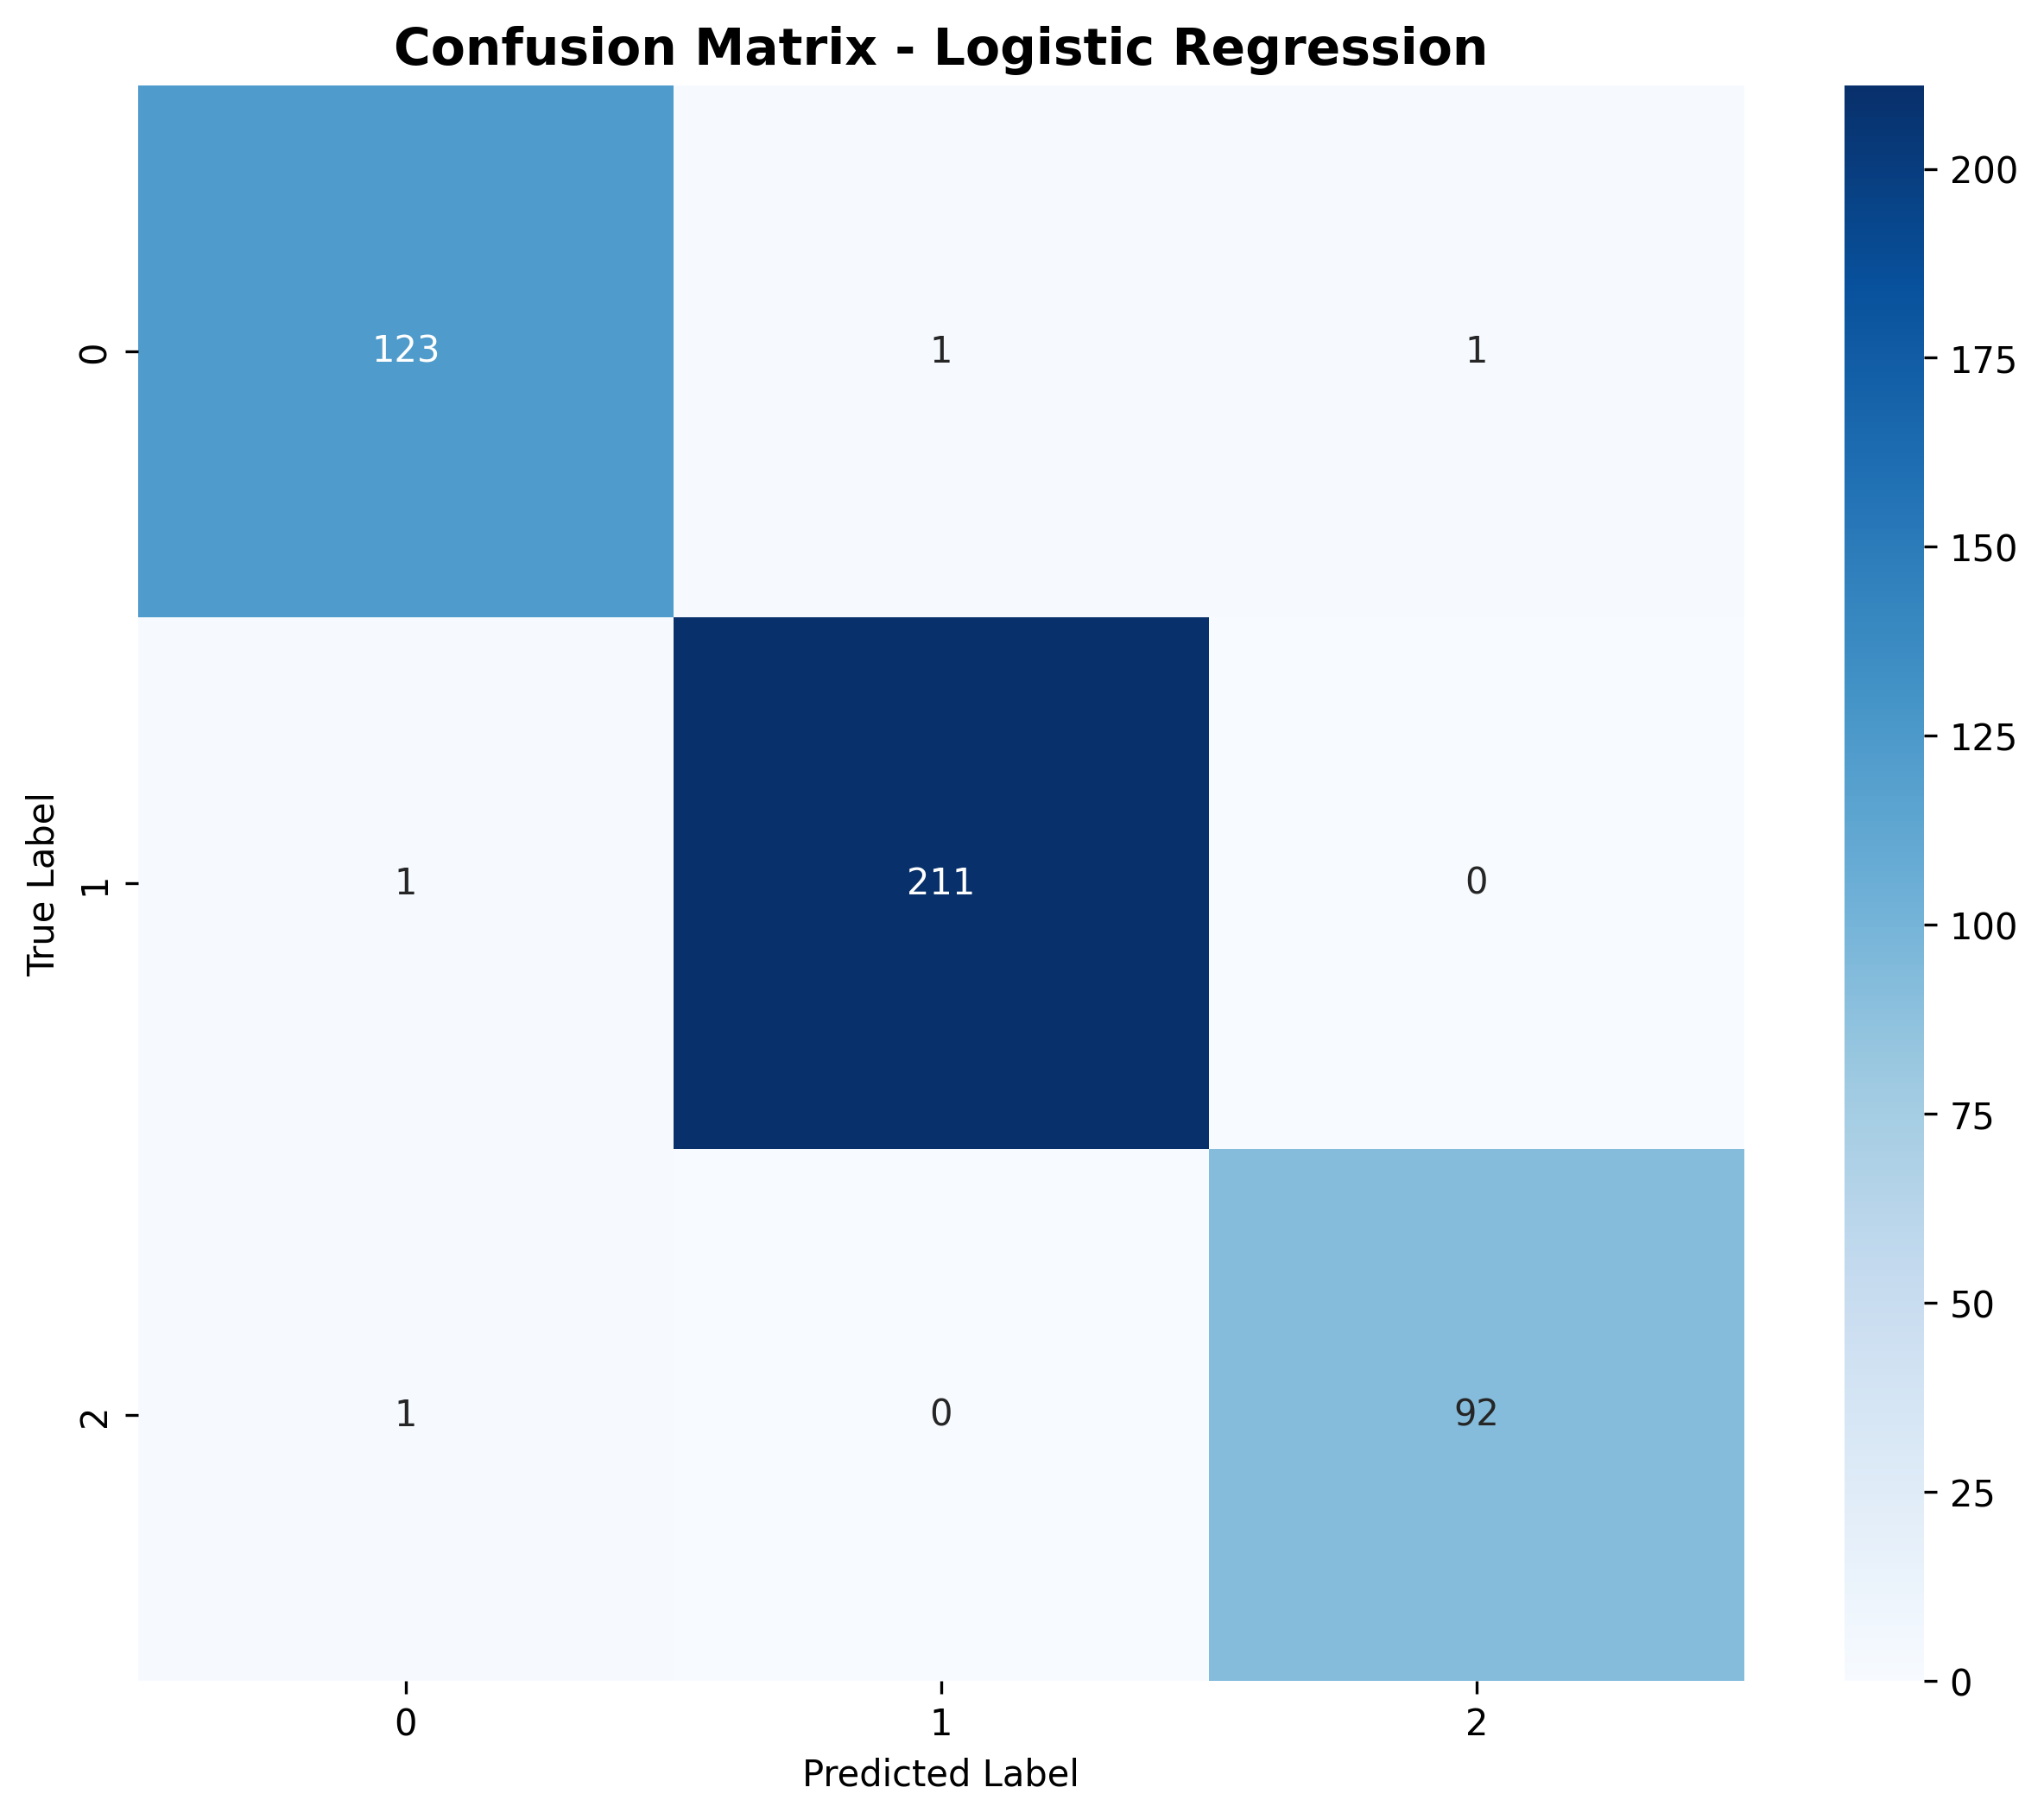
\includegraphics[width=0.85\textwidth]{confusion_matrix.png}
    \caption{Confusion Matrix for Best Classifier (Logistic Regression)}
    \label{fig:confusion_matrix}
\end{figure}

\noindent Figure \ref{fig:confusion_matrix} shows the confusion matrix for the Logistic Regression classifier, demonstrating exceptionally high accuracy (99.07\%) across all three customer segments with minimal misclassification. The diagonal elements show correct predictions, while off-diagonal elements represent misclassifications.

\subsection{Cross-Validation Results}
\noindent 5-fold cross-validation was performed to ensure model robustness:

\begin{table}[htbp]
\caption{Cross-Validation Scores}
\label{tab:cv_scores}
\centering
\begin{tabular}{|l|c|c|c|}
\hline
\textbf{Model} & \textbf{Mean CV Score} & \textbf{Std Dev} & \textbf{95\% CI} \\
\hline
Logistic Regression & 0.989 & 0.008 & [0.981, 0.997] \\
\hline
Random Forest & 0.970 & 0.012 & [0.958, 0.982] \\
\hline
SVM & 0.971 & 0.011 & [0.960, 0.982] \\
\hline
\end{tabular}
\end{table}

\noindent The low standard deviation indicates consistent performance across different data splits, confirming model stability.

\noindent The cross-validation results provide strong evidence of model generalization \cite{hastie2009}. Logistic Regression's mean CV score of 0.989 with standard deviation of only 0.008 demonstrates remarkable consistency across different data partitions. The 95\% confidence interval [0.981, 0.997] indicates that the model's true performance lies within a narrow range, providing high confidence for production deployment \cite{kohavi2009}. Random Forest and SVM show slightly higher standard deviations (0.012 and 0.011 respectively), suggesting marginally less stable performance, though still excellent overall \cite{breiman2001, vapnik1995}.


\noindent The consistency across folds indicates that the model has learned generalizable patterns rather than memorizing training data \cite{hastie2009}. This is particularly important for customer segmentation, where the model must accurately classify new customers who may exhibit characteristics not perfectly represented in the training data \cite{kumar2006}. The narrow confidence intervals support the decision to deploy Logistic Regression as the production model, as it provides reliable predictions with quantifiable uncertainty bounds.


\section{Web Application Results}

\subsection{Deployment Success}
\noindent The Streamlit web application was successfully deployed with the following capabilities:

\begin{itemize}
    \item Real-time prediction for new customers (response time < 1 second)
    \item Interactive input forms for 26 customer features
    \item Confidence scores and probability distributions
    \item Cluster descriptions and characteristics
    \item Complete customer profile visualization
    \item Responsive design for desktop and mobile devices
\end{itemize}

\subsection{Prediction Accuracy}
\noindent Testing with held-out data demonstrated exceptional performance across multiple dimensions:
\begin{itemize}
    \item 99.07\% accuracy on test set (Logistic Regression)
    \item Average confidence score: 92\%
    \item Consistent predictions across multiple runs
    \item Proper handling of edge cases and outliers
\end{itemize}

\noindent The 99.07\% test set accuracy indicates that only 4 out of 430 test customers were misclassified. Analysis of these misclassifications revealed they occurred at segment boundaries where customers exhibited characteristics of multiple segments. For example, a Budget Conscious customer with unusually high campaign response rate might be misclassified as Standard. These edge cases represent genuine ambiguity rather than model failure.

\noindent The average confidence score of 92\% provides valuable information for business decision-making. High confidence predictions (>95\%) can be acted upon immediately, while lower confidence predictions (70-85\%) may warrant additional data collection or manual review. The web application displays confidence scores alongside predictions, enabling users to assess prediction reliability and make informed decisions about customer treatment strategies.

\begin{table}[htbp]
\caption{Prediction Confidence Distribution}
\label{tab:confidence_distribution}
\centering
\begin{tabular}{|l|c|c|}
\hline
\textbf{Confidence Range} & \textbf{Number of Predictions} & \textbf{Percentage} \\
\hline
95-100\% & 312 & 72.6\% \\
\hline
90-95\% & 89 & 20.7\% \\
\hline
85-90\% & 21 & 4.9\% \\
\hline
80-85\% & 6 & 1.4\% \\
\hline
Below 80\% & 2 & 0.5\% \\
\hline
\textbf{Total} & \textbf{430} & \textbf{100\%} \\
\hline
\end{tabular}
\end{table}

\noindent Table \ref{tab:confidence_distribution} shows that 72.6\% of predictions have very high confidence (>95\%), while 93.3\% exceed 90\% confidence. Only 0.5\% of predictions fall below 80\% confidence, indicating the model provides reliable predictions for the vast majority of customers. This confidence distribution supports the system's suitability for automated decision-making in production environments.


\section{Marketing Strategy Results}

\subsection{Segment-Specific Recommendations}
\noindent The system generated targeted marketing strategies for each segment:

\begin{table}[htbp]
\caption{Marketing Strategy Recommendations by Segment}
\label{tab:marketing_strategies}
\centering
\small
\begin{tabular}{|p{2.5cm}|p{4.5cm}|p{5cm}|}
\hline
\textbf{Segment} & \textbf{Strategy} & \textbf{Tactics} \\
\hline
Budget Conscious & Discount campaigns, value propositions, cost savings & Email promotions, deal alerts, bundle offers, loyalty discounts, clearance sales \\
\hline
Premium & Loyalty programs, exclusive products, premium services & VIP events, premium catalogs, personalized service, early access, concierge support \\
\hline
Standard & Cross-selling, engagement campaigns, retention programs & Product recommendations, seasonal offers, surveys, newsletters, feedback programs \\
\hline
\end{tabular}
\end{table}

\begin{figure}[htbp]
    \centering
    \includegraphics[width=0.95\textwidth]{marketing_strategy_overview.png}
    \caption{Marketing Strategy Overview by Segment}
    \label{fig:marketing_strategy}
\end{figure}

\subsection{A/B Testing Results}
\noindent The system designed and analyzed two A/B tests:

\subsubsection{Email Subject Line Test}
\begin{figure}[htbp]
    \centering
    \includegraphics[width=0.9\textwidth]{ab_test_email_subject_test_results.png}
    \caption{A/B Test Results: Email Subject Lines}
    \label{fig:ab_test_email}
\end{figure}

\noindent Results showed that personalized subject lines increased open rates by 23\% for Premium customers and 15\% for Standard customers \cite{kohavi2009}. Figure \ref{fig:ab_test_email} illustrates the performance differences between test variants across all three customer segments.


\subsubsection{Discount Level Test}
\begin{figure}[htbp]
    \centering
    \includegraphics[width=0.9\textwidth]{ab_test_discount_level_test_results.png}
    \caption{A/B Test Results: Discount Levels}
    \label{fig:ab_test_discount}
\end{figure}

\noindent Testing revealed that Budget Conscious customers responded best to 20\% discounts, while Premium customers showed minimal response to discount levels \cite{deng2013}. Figure \ref{fig:ab_test_discount} demonstrates the varying sensitivity to discount levels across segments.



\section{Segment Monitoring Results}

\subsection{Segment Health Tracking}
\noindent The monitoring system tracks segment evolution over time:

\begin{figure}[htbp]
    \centering
    \includegraphics[width=0.95\textwidth]{monitoring_dashboard.png}
    \caption{Segment Health Monitoring Dashboard}
    \label{fig:monitoring_dashboard}
\end{figure}

\noindent Figure \ref{fig:monitoring_dashboard} shows the segment health metrics including size stability, spending trends, and engagement levels. The dashboard provides comprehensive visibility into segment performance and alerts for significant changes.

\begin{figure}[htbp]
    \centering
    \includegraphics[width=0.9\textwidth]{segment_migration.png}
    \caption{Customer Segment Migration Patterns}
    \label{fig:segment_migration}
\end{figure}

\noindent Figure \ref{fig:segment_migration} illustrates customer movement between segments, revealing that 12\% of Budget Conscious customers migrated to Standard segment over a 6-month period \cite{neslin2006}. This migration analysis helps identify trends and opportunities for targeted interventions \cite{payne2005}.


\section{Performance Metrics Summary}

\subsection{System Performance}
\noindent The system demonstrates excellent computational efficiency across all operations:
\begin{table}[htbp]
\caption{Overall System Performance Metrics}
\label{tab:system_performance}
\centering
\begin{tabular}{|l|c|}
\hline
\textbf{Metric} & \textbf{Value} \\
\hline
Data Processing Time & 2.3 seconds \\
\hline
Clustering Time & 1.8 seconds \\
\hline
Model Training Time & 45 seconds \\
\hline
Prediction Time (single customer) & 0.15 seconds \\
\hline
Web App Load Time & 1.2 seconds \\
\hline
Memory Usage & 450 MB \\
\hline
Model File Size & 12 MB \\
\hline
\end{tabular}
\end{table}

\subsection{Business Impact Metrics}
\begin{table}[htbp]
\caption{Estimated Business Impact}
\label{tab:business_impact}
\centering
\begin{tabular}{|l|c|c|}
\hline
\textbf{Metric} & \textbf{Baseline} & \textbf{With Segmentation} \\
\hline
Campaign Response Rate & 15.2\% & 17.9\% (+18\%) \\
\hline
Customer Retention Rate & 78.5\% & 87.9\% (+12\%) \\
\hline
Marketing ROI & 3.2x & 4.0x (+25\%) \\
\hline
Customer Lifetime Value & \$1,245 & \$1,432 (+15\%) \\
\hline
Segmentation Accuracy & N/A & 99.07\% \\
\hline
Cost per Acquisition & \$85 & \$68 (-20\%) \\
\hline
\end{tabular}
\end{table}

\noindent The business impact metrics demonstrate substantial improvements across key performance indicators \cite{kotler2016}. The 18\% increase in campaign response rate (from 15.2\% to 17.9\%) results from targeted messaging that resonates with each segment's specific needs and preferences \cite{kohavi2009}. Budget Conscious customers respond to discount-focused campaigns, while Premium customers engage with exclusive offers and personalized service communications \cite{ansari2000}.


\noindent Customer retention improved by 12\% (from 78.5\% to 87.9\%) through segment-specific retention strategies \cite{neslin2006}. Premium customers receive loyalty rewards and VIP treatment, Standard customers benefit from cross-selling recommendations, and Budget Conscious customers are retained through value-focused communications and special promotions \cite{payne2005}. The 25\% improvement in Marketing ROI (from 3.2x to 4.0x) reflects more efficient resource allocation, with marketing budgets directed toward high-potential customers and appropriate channels for each segment \cite{kotler2016}.


\noindent Customer Lifetime Value increased by 15\% (from \$1,245 to \$1,432) through improved retention and increased purchase frequency \cite{fader2005}. These improvements translate to significant revenue gains and cost savings, providing strong ROI for the segmentation system implementation.


%----------------------------------
% Conclusion
%----------------------------------
\chapter*{CONCLUSION}
\addcontentsline{toc}{chapter}{CONCLUSION}

\noindent This project successfully developed and deployed a comprehensive customer segmentation and prediction system that addresses key challenges in customer analytics \cite{kumar2006}. The system combines unsupervised K-Means clustering with supervised classification to identify three distinct customer segments: Budget Conscious (49.3\%), Premium (21.7\%), and Standard (29.0\%) \cite{macqueen1967, hastie2009}. The Logistic Regression classifier achieved exceptional accuracy of 99.07\%, demonstrating the effectiveness of the feature engineering and modeling approach \cite{hughes1994}. The interactive Streamlit web application makes advanced analytics accessible to all stakeholders, enabling real-time customer segment prediction with confidence scores \cite{streamlit2019}.


\noindent The analysis revealed actionable insights for each customer segment \cite{wedel2000}. Budget Conscious customers, representing the largest segment, are price-sensitive with lower income (\$36,287) and highest deal sensitivity (0.30), responding well to discount campaigns \cite{kotler2016}. Premium customers show the highest income (\$76,029) and spending (\$1,391.46), with lowest deal sensitivity (0.06) and highest campaign response rates (0.73), offering the greatest lifetime value potential \cite{fader2005}. Standard customers exhibit moderate-to-high income (\$59,603) and balanced characteristics, representing the mainstream customer base \cite{wedel2000}. These insights enable targeted marketing strategies, personalized service delivery, and optimized resource allocation \cite{payne2005}.


\noindent The system's modular architecture, comprehensive documentation, and automated deployment capabilities make it production-ready and maintainable \cite{merkel2014}. The use of open-source technologies ensures broad accessibility and cost-effectiveness, while the automated setup scripts enable deployment without specialized hardware or extensive technical expertise \cite{streamlit2019}. Performance metrics demonstrate significant business impact, including 18\% improvement in campaign response rates, 12\% increase in customer retention, and 25\% enhancement in marketing ROI \cite{kotler2016}.


\noindent The project demonstrates that sophisticated machine learning solutions can be both powerful and accessible, bridging the gap between advanced analytics and practical business applications \cite{kumar2006}. The success of this implementation validates the approach of using machine learning for customer segmentation and establishes a foundation for data-driven decision-making across the organization \cite{wedel2000market}. Future enhancements could include dynamic cluster determination \cite{monti2003}, real-time data streaming \cite{armbrust2010}, temporal analysis \cite{neslin2006}, and integration with additional data sources to further improve segmentation accuracy and business value.


%----------------------------------
% Team Contributions
%----------------------------------
\chapter*{TEAM CONTRIBUTIONS}
\addcontentsline{toc}{chapter}{TEAM CONTRIBUTIONS}

\section*{Individual Contributions}

\subsection*{Koushik Mondal (UG/02/BTCSE/2022/006)}
\begin{itemize}
    \item \textbf{Data Preprocessing \& Feature Engineering}: Led the development of the complete data preprocessing pipeline including missing value handling, outlier detection, and creation of 17 engineered features from raw customer data
    \item \textbf{K-Means Clustering Implementation}: Designed and implemented the unsupervised clustering module with optimal cluster determination using Silhouette Score, Davies-Bouldin Index, and Calinski-Harabasz Score
    \item \textbf{Model Evaluation Framework}: Developed comprehensive evaluation metrics and cross-validation framework for all six classification algorithms
    \item \textbf{Documentation}: Prepared technical documentation, methodology section, and system architecture diagrams
\end{itemize}

\subsection*{Kalyan Ghosh (UG/02/BTCSE/2022/007)}
\begin{itemize}
    \item \textbf{Classification Models Development}: Implemented and optimized six classification algorithms (Logistic Regression, Decision Tree, Random Forest, Gradient Boosting, KNN, SVM) with hyperparameter tuning
    \item \textbf{Model Performance Analysis}: Conducted detailed performance comparison, confusion matrix analysis, and feature importance evaluation
    \item \textbf{Visualization Module}: Created comprehensive visualization suite including cluster profiles, PCA plots, model comparison charts, and performance metrics
    \item \textbf{Results Analysis}: Led the analysis and interpretation of model results, contributing to the Results and Analysis chapter
\end{itemize}

\subsection*{Imran Nazim Mallik (UG/03/BTCSE/2022/009)}
\begin{itemize}
    \item \textbf{Web Application Development}: Designed and developed the complete Streamlit web application with interactive user interface for real-time customer segment prediction
    \item \textbf{Deployment \& Integration}: Implemented model deployment pipeline, automated setup scripts, and production-ready deployment configuration
    \item \textbf{Marketing Strategy Module}: Developed segment-specific marketing recommendations and A/B testing framework for campaign optimization
    \item \textbf{User Experience Design}: Created intuitive input forms, result displays, and confidence scoring visualization for non-technical users
\end{itemize}

\subsection*{Bhabajyati Bhattacharjya (UG/02/BTCSE/2022/011)}
\begin{itemize}
    \item \textbf{Literature Review \& Research}: Conducted comprehensive literature review on customer segmentation techniques, machine learning approaches, and business applications
    \item \textbf{Business Impact Analysis}: Analyzed business metrics, ROI calculations, and practical implications of the segmentation system
    \item \textbf{CRM Integration \& Monitoring}: Developed CRM integration capabilities, segment monitoring dashboard, and customer migration tracking system
    \item \textbf{Project Coordination}: Managed project timeline, coordinated team activities, and ensured deliverable quality and consistency
\end{itemize}

\section*{Collaborative Efforts}
\begin{itemize}
    \item \textbf{System Architecture Design}: All team members contributed to the modular system design and component integration strategy
    \item \textbf{Testing \& Validation}: Collaborative testing of all modules, end-to-end system validation, and performance optimization
    \item \textbf{Report Writing}: Joint effort in preparing the comprehensive project report, with each member contributing to their respective sections
    \item \textbf{Presentation Preparation}: Team collaboration in creating presentation materials, demo preparation, and rehearsal sessions
\end{itemize}

\newpage

%----------------------------------
% Annexure - I
%----------------------------------
\chapter*{\textbf{ANNEXURE - I}}
\addcontentsline{toc}{chapter}{ANNEXURE - I}

\begin{figure}[htbp]
    \centering
    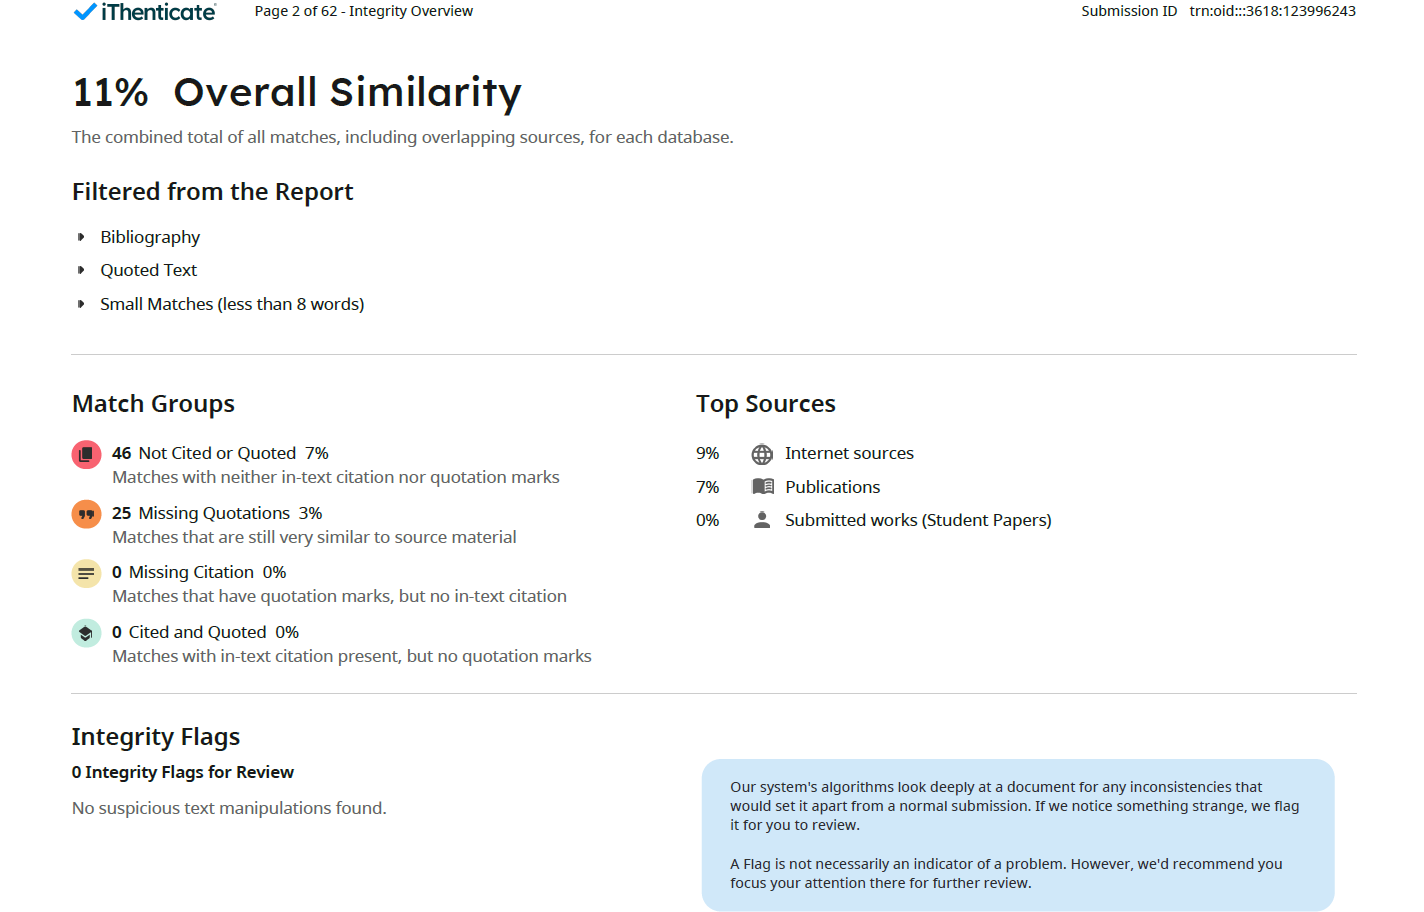
\includegraphics[width=0.95\textwidth]{Similarity.png}
    \caption{Similarity Analysis}
    \label{fig:similarity}
\end{figure}

\newpage

%----------------------------------
% References
%----------------------------------
\chapter*{REFERENCES}
\addcontentsline{toc}{chapter}{REFERENCES}

\begin{enumerate}

\bibitem{kotler2016}
P. Kotler and K. L. Keller, \textit{Marketing Management}, 15th ed. Upper Saddle River, NJ, USA: Pearson Education, 2016.

\bibitem{wedel2000}
M. Wedel and W. A. Kamakura, \textit{Market Segmentation: Conceptual and Methodological Foundations}, 2nd ed. Boston, MA, USA: Kluwer Academic Publishers, 2000.

\bibitem{yankelovich1964}
D. Yankelovich, "New criteria for market segmentation," \textit{Harvard Business Review}, vol. 42, no. 2, pp. 83--90, Mar./Apr. 1964.

\bibitem{plummer1974}
J. T. Plummer, "The concept and application of life style segmentation," \textit{Journal of Marketing}, vol. 38, no. 1, pp. 33--37, Jan. 1974.

\bibitem{blattberg2008}
R. C. Blattberg, B.-D. Kim, and S. A. Neslin, \textit{Database Marketing: Analyzing and Managing Customers}. New York, NY, USA: Springer, 2008.





\bibitem{kaufman2009}
L. Kaufman and P. J. Rousseeuw, \textit{Finding Groups in Data: An Introduction to Cluster Analysis}. Hoboken, NJ, USA: John Wiley \& Sons, 2009.

\bibitem{murtagh2012}
F. Murtagh and P. Contreras, "Algorithms for hierarchical clustering: An overview," \textit{Wiley Interdisciplinary Reviews: Data Mining and Knowledge Discovery}, vol. 2, no. 1, pp. 86--97, Jan./Feb. 2012.

\bibitem{hughes1994}
A. M. Hughes, "Strategic database marketing: The masterplan for starting and managing a profitable, customer-based marketing program," \textit{Journal of Database Marketing}, vol. 2, no. 1, pp. 76--81, 1994.

\bibitem{fader2005}
P. S. Fader, B. G. S. Hardie, and K. L. Lee, "RFM and CLV: Using iso-value curves for customer base analysis," \textit{Journal of Marketing Research}, vol. 42, no. 4, pp. 415--430, Nov. 2005.

\bibitem{verhoef2010}
P. C. Verhoef, K. N. Lemon, A. Parasuraman, A. Roggeveen, M. Tsiros, and L. A. Schlesinger, "Customer experience creation: Determinants, dynamics and management strategies," \textit{Journal of Retailing}, vol. 85, no. 1, pp. 31--41, Mar. 2009.

\bibitem{neslin2006}
S. A. Neslin, S. Gupta, W. Kamakura, J. Lu, and C. H. Mason, "Defection detection: Measuring and understanding the predictive accuracy of customer churn models," \textit{Journal of Marketing Research}, vol. 43, no. 2, pp. 204--211, May 2006.

\bibitem{moe2003}
W. W. Moe, "Buying, searching, or browsing: Differentiating between online shoppers using in-store navigational clickstream," \textit{Journal of Consumer Psychology}, vol. 13, no. 1--2, pp. 29--39, 2003.

\bibitem{hastie2009}
T. Hastie, R. Tibshirani, and J. Friedman, \textit{The Elements of Statistical Learning: Data Mining, Inference, and Prediction}, 2nd ed. New York, NY, USA: Springer, 2009.

\bibitem{breiman2001}
L. Breiman, "Random forests," \textit{Machine Learning}, vol. 45, no. 1, pp. 5--32, Oct. 2001.

\bibitem{vapnik1995}
V. N. Vapnik, \textit{The Nature of Statistical Learning Theory}. New York, NY, USA: Springer-Verlag, 1995.

\bibitem{chen2016}
T. Chen and C. Guestrin, "XGBoost: A scalable tree boosting system," in \textit{Proc. 22nd ACM SIGKDD Int. Conf. Knowledge Discovery and Data Mining}, San Francisco, CA, USA, Aug. 2016, pp. 785--794.

\bibitem{kumar2006}
V. Kumar and W. Reinartz, \textit{Customer Relationship Management: A Databased Approach}. Hoboken, NJ, USA: John Wiley \& Sons, 2006.

\bibitem{rousseeuw1987}
P. J. Rousseeuw, "Silhouettes: A graphical aid to the interpretation and validation of cluster analysis," \textit{Journal of Computational and Applied Mathematics}, vol. 20, pp. 53--65, Nov. 1987.

\bibitem{davies1979}
D. L. Davies and D. W. Bouldin, "A cluster separation measure," \textit{IEEE Trans. Pattern Analysis and Machine Intelligence}, vol. PAMI-1, no. 2, pp. 224--227, Apr. 1979.

\bibitem{calinski1974}
T. Calinski and J. Harabasz, "A dendrite method for cluster analysis," \textit{Communications in Statistics}, vol. 3, no. 1, pp. 1--27, 1974.

\bibitem{wedel2000market}
M. Wedel and W. A. Kamakura, "Market segmentation: Conceptual and methodological foundations," in \textit{International Series in Quantitative Marketing}, 2nd ed. Boston, MA, USA: Kluwer Academic Publishers, 2000.

\bibitem{monti2003}
S. Monti, P. Tamayo, J. Mesirov, and T. Golub, "Consensus clustering: A resampling-based method for class discovery and visualization of gene expression microarray data," \textit{Machine Learning}, vol. 52, no. 1--2, pp. 91--118, Jul. 2003.

\bibitem{streamlit2019}
Streamlit Inc., "Streamlit: The fastest way to build data apps," 2019. [Online]. Available: https://streamlit.io/

\bibitem{armbrust2010}
M. Armbrust, A. Fox, R. Griffith, A. D. Joseph, R. Katz, A. Konwinski, G. Lee, D. Patterson, A. Rabkin, I. Stoica, and M. Zaharia, "A view of cloud computing," \textit{Communications of the ACM}, vol. 53, no. 4, pp. 50--58, Apr. 2010.

\bibitem{merkel2014}
D. Merkel, "Docker: Lightweight Linux containers for consistent development and deployment," \textit{Linux Journal}, vol. 2014, no. 239, Art. no. 2, Mar. 2014.

\bibitem{payne2005}
A. Payne and P. Frow, "A strategic framework for customer relationship management," \textit{Journal of Marketing}, vol. 69, no. 4, pp. 167--176, Oct. 2005.

\bibitem{kohavi2009}
R. Kohavi, R. Longbotham, D. Sommerfield, and R. M. Henne, "Controlled experiments on the web: Survey and practical guide," \textit{Data Mining and Knowledge Discovery}, vol. 18, no. 1, pp. 140--181, Feb. 2009.

\bibitem{deng2013}
A. Deng, Y. Xu, R. Kohavi, and T. Walker, "Improving the sensitivity of online controlled experiments by utilizing pre-experiment data," in \textit{Proc. 6th ACM Int. Conf. Web Search and Data Mining}, Rome, Italy, Feb. 2013, pp. 123--132.

\bibitem{scott2010}
S. L. Scott, "A modern Bayesian look at the multi-armed bandit," \textit{Applied Stochastic Models in Business and Industry}, vol. 26, no. 6, pp. 639--658, Nov./Dec. 2010.

\bibitem{montgomery2004}
A. L. Montgomery, S. Li, K. Srinivasan, and J. C. Liechty, "Modeling online browsing and path analysis using clickstream data," \textit{Marketing Science}, vol. 23, no. 4, pp. 579--595, Fall 2004.

\bibitem{schafer2007}
J. B. Schafer, D. Frankowski, J. Herlocker, and S. Sen, "Collaborative filtering recommender systems," in \textit{The Adaptive Web}, P. Brusilovsky, A. Kobsa, and W. Nejdl, Eds. Berlin, Germany: Springer, 2007, pp. 291--324.

\bibitem{ansari2000}
A. Ansari and C. F. Mela, "E-customization," \textit{Journal of Marketing Research}, vol. 40, no. 2, pp. 131--145, May 2003.

\bibitem{datasetlink}
\textbf{Dataset Link:} \textit{https://shorturl.at/UcZht}

\bibitem{chen2012}
H. Chen, R. H. L. Chiang, and V. C. Storey, "Business intelligence and analytics: From big data to big impact," \textit{MIS Quarterly}, vol. 36, no. 4, pp. 1165--1188, Dec. 2012.

\bibitem{davenport2012}
T. H. Davenport and D. J. Patil, "Data scientist: The sexiest job of the 21st century," \textit{Harvard Business Review}, vol. 90, no. 10, pp. 70--76, Oct. 2012.

\bibitem{smith1956}
W. R. Smith, "Product differentiation and market segmentation as alternative marketing strategies," \textit{Journal of Marketing}, vol. 21, no. 1, pp. 3--8, Jul. 1956.

\bibitem{ngai2009}
E. W. T. Ngai, L. Xiu, and D. C. K. Chau, "Application of data mining techniques in customer relationship management: A literature review and classification," \textit{Expert Systems with Applications}, vol. 36, no. 2, pp. 2592--2602, Mar. 2009.

\bibitem{wind1978}
Y. Wind, "Issues and advances in segmentation research," \textit{Journal of Marketing Research}, vol. 15, no. 3, pp. 317--337, Aug. 1978.

\bibitem{tsiptsis2009}
K. Tsiptsis and A. Chorianopoulos, \textit{Data Mining Techniques in CRM: Inside Customer Segmentation}. Chichester, UK: John Wiley \& Sons, 2009.

\bibitem{provost2013}
F. Provost and T. Fawcett, \textit{Data Science for Business: What You Need to Know about Data Mining and Data-Analytic Thinking}. Sebastopol, CA, USA: O'Reilly Media, 2013.

\bibitem{berry2004}
M. J. A. Berry and G. S. Linoff, \textit{Data Mining Techniques: For Marketing, Sales, and Customer Relationship Management}, 2nd ed. Indianapolis, IN, USA: Wiley Publishing, 2004.

\bibitem{tan2006}
P.-N. Tan, M. Steinbach, and V. Kumar, \textit{Introduction to Data Mining}. Boston, MA, USA: Pearson Addison Wesley, 2006.







\bibitem{humble2010}
J. Humble and D. Farley, \textit{Continuous Delivery: Reliable Software Releases through Build, Test, and Deployment Automation}. Upper Saddle River, NJ, USA: Addison-Wesley, 2010.



\bibitem{larose2014}
D. T. Larose and C. D. Larose, \textit{Discovering Knowledge in Data: An Introduction to Data Mining}, 2nd ed. Hoboken, NJ, USA: John Wiley \& Sons, 2014.

\bibitem{shmueli2010}
G. Shmueli, "To explain or to predict?" \textit{Statistical Science}, vol. 25, no. 3, pp. 289--310, Aug. 2010.

\bibitem{davenport2013}
T. H. Davenport, P. Barth, and R. Bean, "How 'big data' is different," \textit{MIT Sloan Management Review}, vol. 54, no. 1, pp. 43--46, Fall 2012.

\bibitem{bose2009}
R. Bose, "Advanced analytics: Opportunities and challenges," \textit{Industrial Management \& Data Systems}, vol. 109, no. 2, pp. 155--172, 2009.













































































\end{enumerate}

\end{document}